%% Copyleft 2018 Jean-Baptiste Louvet
%% Copyright (C) 2014 Dorian Depriester
%% http://blog.dorian-depriester.fr
%%
%% This file may be distributed and/or modified under the conditions
%% of the LaTeX Project Public License, either version 1.3c of this
%% license or (at your option) any later version. The latest version
%% of this license is in:
%%
%%    http://www.latex-project.org/lppl.txt
%%
%% and version 1.3c or later is part of all distributions of LaTeX
%% version 2006/05/20 or later.
%%
%% This work has the LPPL maintenance status `maintained'.
%%
%% The Current Maintainer of this work is Dorian Depriester
%% <contact [at] dorian [-] depriester [dot] fr>.
%%
%% This is main.tex for French PhD Thesis.
%% See http://blog.dorian-depriester.fr/latex/template-these/template-complet-pour-manuscrit-de-these for help


%%%%%%%%%%%%%%%%%%%%%%%%%%%%%%%%%%%%%%%%%
%           Fichier maitre				%
%%%%%%%%%%%%%%%%%%%%%%%%%%%%%%%%%%%%%%%%%

\documentclass[a4paper, english, 11pt, twoside,openright]{report}
\input{Preambule}		% Liste des packages et de leurs options
%%%%%%%%%%%%%%%%%%%%%%%%%%%%%%%%%%%%%%%%
%           Commandes perso            %
%%%%%%%%%%%%%%%%%%%%%%%%%%%%%%%%%%%%%%%%

%% Figures centrées, et en position 'here, top, bottom or page'
\newenvironment{figureth}{%
		\begin{figure}[htbp]
			\centering
	}{
		\end{figure}
		}
		
		
%% Tableaux centrés, et en position 'here, top, bottom or page'
\newenvironment{tableth}{%
		\begin{table}[htbp]
			\centering
			%\rowcolors{1}{coleurtableau}{coleurtableau}
	}{
		\end{table}
		}

%% Sous-figures centrées, en position 'top'		
\newenvironment{subfigureth}[1]{%
	\begin{subfigure}[t]{#1}
	\centering
}{
	\end{subfigure}
}

\newcommand{\citationChap}[2]{%
	\epigraph{\og \textit{#1} \fg{}}{#2}
}

%% On commence par une page impaire quand on change le style de numérotation de pages 
\let\oldpagenumbering\pagenumbering
\renewcommand{\pagenumbering}[1]{%
	\cleardoublepage
	\oldpagenumbering{#1}
}

\newcommand{\GG}[1]{{\color{red} GG:  #1}}
\newcommand{\CR}[1]{{\color{blue} CR:  #1}}
\newcommand{\RH}[1]{{\color{green} RB:  #1}}

\newenvironment{chapterabstract}{{\center \Large \textbf{\textit{Chapter abstract}}\vspace{0.3cm}\\}\rightskip1in\itshape}{}

\newcommand{\cmark}{\ding{51}}%
\newcommand{\xmark}{\ding{55}}%

\newcommand{\setS}{\mathcal{S}}
\newcommand{\setX}{\mathcal{X}}
\newcommand{\setY}{\mathcal{Y}}
\newcommand{\setZ}{\mathcal{Z}}
\newcommand{\trainsetX}{\mathcal{D}_X}
\newcommand{\trainsetY}{\mathcal{D}_Y}
\newcommand{\vect}{\text{vect}}

\makeatletter
\newcommand{\acronym}[2]{
	\label{acronyms:#1}
	\expandafter\newcommand\csname#1\endcsname {#1}%
	#1 & #2 \\
}
\makeatother

	% Commandes et environnements perso
\input{PageDeGarde}


% Méta-données du PDF
\hypersetup{
    pdfauthor={Cyprien Ruffino},
    pdfsubject={Manuscrit de thèse de doctorat},
    pdftitle={Auxiliary Tasks for the Conditioning of Generative Adversarial Networks},
    pdfkeywords={TODO}%TODO
}


%%%%%%%%%%%%%%%%%%%%%%%%%%%%%%%%%%%%%%%%%%%%%%%%%%%%%%%%%%%%%%%%%
%%   			Liste des fichiers à compiler					%
%%%%%%%%%%%%%%%%%%%%%%%%%%%%%%%%%%%%%%%%%%%%%%%%%%%%%%%%%%%%%%%%%
%	\includeonly{Chapitre1,Chapitre2,Annexes}


% Répertoire contenant les images
\graphicspath{{images/}}
% Infos de la page de garde
\author{Cyprien \textsc{Ruffino}}
\title{Auxiliary Tasks for the Conditioning of Generative Adversarial Networks}
\specialite{Informatique}
\ecole{l'\'Ecole Doctorale Mathématiques, Information, Ingéniérie des Systèmes}
\date{\today}
\directeur{Gilles \textsc{Gasso}}
\encadrant{Romain \textsc{Hérault}} %Optionnel
\jurya{Civilité / prénom \textsc{Nom}}{Grade / fonction / statut / lieu d'exercice}{Rapporteur ou examinateur ou directeur de thèse ou codirecteur de thèse}
\juryb{Civilité / prénom \textsc{Nom}}{Grade / fonction / statut / lieu d'exercice}{Rapporteur ou examinateur ou directeur de thèse ou codirecteur de thèse}
\juryc{Civilité / prénom \textsc{Nom}}{Grade / fonction / statut / lieu d'exercice}{Rapporteur ou examinateur ou directeur de thèse ou codirecteur de thèse}
\juryd{Civilité / prénom \textsc{Nom}}{Grade / fonction / statut / lieu d'exercice}{Rapporteur ou examinateur ou directeur de thèse ou codirecteur de thèse}
\jurye{Civilité / prénom \textsc{Nom}}{Grade / fonction / statut / lieu d'exercice}{Rapporteur ou examinateur ou directeur de thèse ou codirecteur de thèse}

\newcommand{\ver}{0.0}% Version du document

\pagestyle{fancy}
\begin{document}
% Préambule
	\pagenumbering{roman}
	\pagedegarde
	\cleardoublepage
			\setcounter{tocdepth}{2}
			
			\dominitoc
			\tableofcontents
			\renewcommand*\listfigurename{List of figures}
			\listoffigures
			\renewcommand*\listtablename{List of tables}
			\listoftables
			

%%%%%%%%%%%%%%%%%%%%%%%%%%%%%%%%%%%%%		
%        Contenu du document        %
%%%%%%%%%%%%%%%%%%%%%%%%%%%%%%%%%%%%%
	\setcounter{mtc}{3}	% "Corrige" les minitocs décallés à cause des chapter* (ex : table des matières)
	\pagenumbering{arabic}

\chapter*{Abstract}
%\addcontentsline{toc}{chapter}{Abstract}
\label{chap:abstract}

During the last decade, Generative Adversarial Networks (\ac{GANs}) have caused a tremendous leap forward in image generation as a whole. Their ability to learn very complex, high-dimension distributions not only had a huge impact on the field of generative modeling, their influence extended to the general public at large. By being the first models able generate high-dimension photo-realistic images, \ac{GANs} very quickly gained popularity as an image generation and photo manipulation technique. For example, their use as "filters" became common practice on social media, but they also allowed for the rise of \textit{Deepfakes}, images that have been manipulated in order to fake the identity of a person. 

In this thesis, we explore the conditioning of Generative Adversarial Networks, that is influencing the generation process in order to control the content of a generated image. We focus on conditioning through auxiliary tasks, that is we  explicitly implement additional objective to the generative model to complement the initial goal of learning the data distribution.

First, we introduce generative modeling through several examples, and present the Generative Adversarial Networks framework. We discuss theoretical interpretations of \ac{GANs} as well as its most prominent issues, notably the lack of stability during training of the model and the difficulty to generate diverse samples. We review classical techniques for conditioning GANs and propose an overview of recent approaches aiming to both solve the aforementioned issues and enhance the visual quality of the generated images.

Afterwards, we focus on a specific generation task that requires conditioning: image reconstruction. In a nutshell, the problem consists in recovering an image from which we only have a handful of pixels available, usually around 0.5\%. It stems from an application in geostatistics, namely the reconstruction of underground terrain from a reduced amount of expensive and difficult to obtain measurements. To do so, we propose to introduce an explicit auxiliary reconstruction task to the GAN framework which, in addition to a diversity-restoring technique, allows for the generation of high-quality images that respect the given measurements.

Finally, we investigate a task of domain-transfer with generative models, specifically transferring images from the \ac{RGB} color domain to the polarimetric domain. Polarimetric images bear hard constraints that directly stem from the physics of polarimetry. Leveraging on the cyclic-consistency paradigm, we extend the training of generative models with auxiliary tasks that push the generator towards enforcing the polarimetric constraints. We highlight that the approach manages to generate physically realistic polarimetric images. Empirical evidence illustrates that using the generated images as  data augmentation improves the performance on object detection models for road scene analysis.
\chapter*{Résumé}
%\addcontentsline{toc}{chapter}{Résumé}
\label{chap:resume}

\begin{otherlanguage}{french}
Au cours de la dernière décennie, les réseaux génératifs antagonistes (Generative Adversatial Networks, ou \ac{GAN}s) ont révolutionné la génération d'images dans son ensemble. Leur capacité à apprendre des distributions très complexes en grande dimension ils ont eu eu un impact important sur le domaine des modèles génératifs et leur influence s'est largement étendue au grand public. En effet, en étant les premiers modèles capables de générer des images photo-réalistes en haute dimension, ils ont très vite gagné en popularité en tant que technique de génération d'images et de manipulation de photos. Par exemple, leur utilisation en tant que "filtres" est devenue une pratique courante sur les médias sociaux: ils ont également permis l'essor des \textit{Deepfakes}, des images manipulées afin de falsifier l'identité d'une personne. 

Dans cette thèse, nous étudions le conditionnement des réseaux génératifs antagonistes, c'est-à-dire influencer le processus de génération afin de contrôler le contenu d'une image générée. Nous nous concentrons sur le conditionnement par le biais de tâches auxiliaires, c'est-à-dire l'utilisation d'un ou plusieurs objectifs supplémentaires au modèle génératif en plus de l'objectif initial d'apprentissage de la distribution des données.

Nous introduisons les principes de la modélisation générative à travers plusieurs  exemples, et nous présentons le cadre des réseaux génératifs antagonistes. Nous analysons les interprétations théoriques de ce modèle ainsi que ses problèmes les plus importants, notamment l'instabilité de l'apprentissage du modèle et la difficulté de générer des échantillons diversifiés. Nous passons en revue les techniques classiques de conditionnement des GAN et proposons un aperçu des approches récentes visant à résoudre ses problèmes et à améliorer la qualité visuelle des images générées.

Dans la suite de la thèse, nous nous concentrons sur une tâche de génération spécifique qui nécessite un conditionnement : la reconstruction d'images. Ce problème consiste à générer une image dont nous ne connaissons qu'un nombre très réduit de pixels à priori, généralement autour de 0,5 \%. Ceci est motivé par une application directe en géostatistique : la reconstruction de données géologiques de sous-sols à partir d'une très petite quantité de mesures coûteuses et difficiles à obtenir. Pour ce faire, nous proposons d'introduire une tâche de reconstruction auxiliaire explicite dans le cadre du GAN qui, combinée à une technique de restauration de la diversité, a permis de générer des images de haute qualité qui respectent les mesures données.

Dans la deuxième contribution nous étudions une tâche de transfert de domaine avec des modèles génératifs, en particulier le transfert d'images du domaine couleur au domaine polarimétrique. Les images polarimétriques sont soumises à des contraintes strictes qui découlent directement des proprétés physiques de la polarimétrie. En s'appuyant sur l'approche de cohérence cyclique, nous étendons la formulation des modèles génératifs avec des tâches auxiliaires qui poussent le générateur à faire respecter les contraintes polarimétriques. Nous montrons que cette approche permet non seulement de générer des images polarimétriques physiquement réalistes, mais que l'utilisation des images générées comme données augmentées augmente la performance des modèles de détection d'objets sur des applications d'analyse de scène routière.
\end{otherlanguage}

\chapter*{Introduction}
\fancyhead[R]{\textit{INTRODUCTION}}
\addcontentsline{toc}{chapter}{Introduction}
\label{chap:intro}

\section*{Context}
\addcontentsline{toc}{section}{Context}

Over the last decade, deep learning has emerged as one of the most promising areas of artificial intelligence, progressively equaling or surpassing all traditional approaches in several fields of application. Thanks to the generalization capacity of deep neural networks, it is able to leverage large amounts of data to learn complex patterns and behaviors. Deep learning has been applied successfully to diverse domains such as machine translation, the game of go and high-frequency trading. Among all these application domains, computer vision is surely the one in which deep learning has had the greatest impact. Consisting in analyzing and processing images automatically, computer vision is a complex field that contains many problems such as object detection or pattern recognition. Nowadays, deep learning is the reference approach for all computer vision tasks and is used in areas such as medical imaging, facial recognition and autonomous driving.

One of the sub-domains of computer vision that emerged thanks to deep learning is automatic image generation. Generative Adversarial Networks (\ac{GANs}) \citep{Goodfellow2014} are now the spearhead of deep learning for image generation. They were made famous during recent years for their ability to generate photo-realistic images\footnote{A striking example : \url{https://www.whichfaceisreal.com/}}. Indeed, by allowing for the generation of high quality and high dimensional images, they have quickly found applications in many domains such as increasing image resolution \citep{Wang2020}, cartography \citep{Kang2019}, video completion \citep{Vondrick2016} or automatic  3D objects generation \citep{Wu2017}. The use of \ac{GANs} has also been extended to application targeting the public at large, such as the numerous "filters" available on social networks, allowing for example to edit pictures of a person to make them look older \citep{Antipov2017a}. \ac{GANs} also lead to some more harmful applications, such as the famous "deepfakes" \citep{Vaccari2020} that automatically generates images and videos whose purpose is to deceive by falsifying the identity of a person, most often a celebrity or a politician.

In this thesis, we propose to study auxiliary tasks for the conditioning of generative adversarial networks. While \ac{GANs} excel in image generation and allow for generating very high quality images, they only reach their full potential when they are conditioned, i.e. when it is possible to control the model output. Indeed, the conditioning makes it possible to ensure that the obtained images have desired properties, which is essential for, for example, all dynamic image editing applications such as "filters" or the increase in resolution. Indeed, the content of the image, for example the person on which the filter is applied, must remain the same. We therefore propose to focus on a family of techniques conditioning \ac{GANs}: auxiliary tasks. By training a \ac{GAN} to solve a secondary task, simultaneously to learning the distribution of real data, it is possible to push the model towards respecting some targeted properties. These auxiliary tasks need to be designed specifically for each type of conditioning. Over the course of this thesis, we will examine examples of problems that can be solved by conditioned generative models and will propose appropriate auxiliary tasks to solve these problems.


\section*{Motivations}
\addcontentsline{toc}{section}{Motivations}

Our work is motivated by two applications requiring conditioned generative models: the reconstruction of images, and more precisely maps of underground water channel formations; and the conversion of road scene \ac{RGB} image databases into the polarimetric domain. 

\subsection*{Reconstruction of hydro-geological images}

\quad First, we study the problem of image reconstruction, consisting in (re-)generating an image from a very reduced set of a priori known pixels. This is a generic task which includes the problem of reconstructing maps of underground water channel formations. Within this application, we seek several properties:

\textbf{Pixel precise.} Since the task of image reconstruction consists in generating an image from which precisely-positioned pixels are pre-drawn, their positions and values must be preserved in the resulting image. In the context of the geology application, this implies preserving precisely the position and value of the real measurements made on the field.

\textbf{Preserves diversity.} One of the limitations of \ac{GANs} is their tendency to loose the ability to generate diverse samples, and thus they produce images that are very close to each other. In geological applications, it is important to be able to produce a large number of diverse candidate images that fulfill the pre-drawn pixels.

\textbf{Fast generation process.} In order to be able to generate a large number of candidate images, it is also important that the generation process is fast. Thus, existing approaches that require solving an optimization problem for each generated image will most often be far too slow to be applicable here.

\subsection*{Polarimetric Image Conversion}

\quad In a second step, we address the problem of polarimetric image generation as a data augmentation technique. Indeed, the lack of labeled polarimetric data is a major impediment to research in the field of computer vision in polarimetric images. These images, capturing properties of light that are not present in color images, allow, for example, for better results in detection tasks in adverse weather conditions such as heavy rain or fog. By transferring labeled databases from the color image domain to the polarimetric domain, this shortage of labeled polarimetric data could be circumvented. However, there are several requirements that must be met:

\textbf{Respect of polarimetric constraints.} Polarimetric imaging is subject to strong constraints emanating from the wave physics of light. These constraints must be taken into account in order to generate images that are not only realistic, but above also the physical properties that may allow improved detection results in adverse weather conditions.

\textbf{Respect of the polarimetric camera calibration.} In order to capture polarimetric images, a dedicated camera uses a number of filters that let polarized light pass through at predefined angles. The configuration of these filters may differ depending on the used camera. The calibration directly affects the nature of the acquired images. Thus, when generating polarimetric data, it is necessary to ensure that the produced images correspond to the calibration of the used camera.

\textbf{Preserves the image content.} The objective of this application is to produce synthetic labeled datasets by transferring existing labeled datasets into the polarimetric domain. In order to be able to preserve the labels between these two domains, it is therefore necessary that the image content remains similar in nature and position.

\textbf{Quick generation process.} In order to be able to transfer entire databases into the polarimetric domain, it is also necessary that the image generation time is not too high, since these databases may contain several hundreds of thousands of high-resolution images. High generation times would thus make the approach prohibitively expensive.

\section*{Outline and contributions}
\addcontentsline{toc}{section}{Outline and contributions}

Since conditioning generative models is a crucial step for applying them to real-world problems, in this thesis we study the conditioning of Generative Adversarial Networks, most notably using auxiliary tasks. The thesis is composed of three chapters, whose contents are detailed below, as well as a conclusion.

\subsection*{Chapter 1: Introduction to Generative Adversarial Networks}

We begin the thesis with an introduction chapter on Generative Adversarial Networks (GANs), a framework for training deep neural networks as generative models that is particularly well suited for image generation. We  highlight their limitations, most notably the instability of the training process and the lack of diversity in the generated data. We investigate its conditional variants. These allow for exerting some control over the generation process by applying constraints on the generated data, as well as domain transfer approaches, the task of projecting data from one domain to another (e.g., converting a painting into a photo).  We present an overview of the different techniques used to counteract the limitations of GANs by improving the neural network architecture and changing the cost function of the GAN. Finally, we conclude this chapter by discussing the difficulties involved in evaluating generative models and examine the most commonly used metrics for evaluating GANs.

\subsection*{Chapter 2: Image reconstruction as an auxiliary task to generative modeling}

In this chapter, we propose an overview of the task of reconstructing altered images with generative models. As a contribution to this problem, we propose an approach for conditioning \ac{GANs} using an explicit auxiliary reconstruction task. Combined with a technique for limiting the diversity-loss issues, optimizing this auxiliary task during the training process, the obtained models are able to quickly reconstruct images, in comparison to similar methods, such as compressed sensing-based approaches, that need to solve an optimization problem for each reconstructed image.  A byproduct of our approach is a hyper-parameter that controls the impact of the reconstruction loss on the generative model. We show that this hyper-parameter directly influences a trade-off between the fidelity of the reconstruction and visual quality of the generated images.

We evaluate our approach on several image reconstruction tasks using classical image datasets such as MNIST or CIFAR10, as well as a texture image dataset. Finally, we apply this method to a geology problem, namely reconstructing underground water channels formations using very few points. Empirical results show that our approach equals or outperforms existing approaches while providing the ability to control the trade-off between the visual quality and the fulfillment of the constraints.

\subsection*{Chapter 3: Domain-transfer with auxiliary tasks for generative modeling}

In this chapter, we study the conditioning of domain-transfer models that makes use of Generative Adversarial Networks. Such models, usually revolving around the idea of cycle-consistency, allow for transferring images from one "domain" to the other without the used of paired data, which is usually very hard to obtain. We focus on the task of transferring a color image to the polarimetric domain. Such images bear hard constraints that directly stem from the physics of light, thus unconstrained domain-transfer approaches cannot solve this problem by themselves. 

We introduce new auxiliary tasks based on a reformulation of these constraints and propose an algorithm to integrate them to the training of a domain-transfer model. We show that this method performs well on a polarimetric image generation task, both in term of visual quality and respect of the constraints.

Finally, we apply this approach to a data-augmentation task. Indeed, no large polarimetric images datasets are publicly available at the time of writing this thesis, so training deep models to solve problems on polarimetric images is difficult. By transferring color-images labeled datasets to the polarimetric images domain, we can produce large datasets of labeled polarimetric images. We show that such a dataset increases the performance of a detection network in polarimetric images.


\section*{Related publications}
\addcontentsline{toc}{section}{Related publications}

\begin{itemize}
	\item\longfullcite{Ruffino2017}
	\item\longfullcite{Ruffino2019a}
	\item\longfullcite{Laloy2019}
	\item\longfullcite{Ruffino2020}
	\item\longfullcite{Blin2021}
\end{itemize}


\fancyhead[R]{}
\chapter{Introduction to Generative Adversarial Networks }
\label{chap:chapter1}

\begin{chapterabstract}
	In this chapter, we first propose an introduction to the problem of generative modeling and some solutions to tackle this problem. We then propose an overview of the Generative Adversarial Networks \citep{Goodfellow2014} framework, which is a recent method to train deep neural networks as generative models that is particularly adapted to the task of image generation. We will introduce some of its theoretical interpretations, as well as some of its variations and applications. We discuss the different limitations of this approach and expose three main goals among the different works: enhancing the visual quality of the generated samples; maintaining their diversity; and conditioning the model. We then discuss the recent advances that have been made to overcome some of these limitations and propose a taxonomy of these advances using the aforementioned directions. We discuss the evaluation of generative models and the difficulties of evaluating the intrinsic quality of a generated sample through an overview of the different classical metrics and discuss their limitations.
\end{chapterabstract}

\minitoc


\section{Generative modeling with Adversarial models}
Generative modeling with deep neural networks has been a challenging task due to the stochastic nature of sampling, which prevents the computation of gradient, thus preventing the classical training of a deep model with gradient descent. However recent approaches such as variational autoencoders (\ac{VAE}s) \citep{Kingma2014b}, flow methods \citep{Dinh2017, Kingma2018} and adversarial models \citep{Goodfellow2014} managed to overcome this restriction. In this section, we first propose an introduction to generative modeling with a focus on latent variable models.

We will then focus on the Generative Adversarial Networks \citep{Goodfellow2014} framework, their training process  and some of their variants, especially their conditional and domain-transfer variants. We outline some limitations of this framework and propose a formulation of these limitations in the form of a trilemma between the intrinsic quality of the generated samples, their diversity and the quality of the conditioning of the model. With this tool, we propose a taxonomy of the recent \ac{GAN} approaches and identify trends in these approaches.


\subsection{Generative modeling with maximum likelihood estimation}

\begin{figure}
	\centering
	\includegraphics[width=\textwidth*3/4]{chapter1/disc_gen.pdf}
	\caption[Generative modeling]{Left: Discriminative modeling, the model aims to assign a class to each data point. Right: Generative modeling, the model aims to learn the underlying probability distribution of the data points.}
	\label{fig:disc_gen}
\end{figure}

Generative modeling is the task of learning the underlying distribution of a dataset in order to generate more samples from that distribution. In other words, it describes how data is generated in terms of a probabilistic model,  a distribution from which the whole dataset could have been sampled with a high likelihood.

 Indeed,  whereas a discriminative model tries to find decision boundaries by fitting a parametric model $\pt{\vy|\vx}$  to a conditional probability distribution $\p{\vy|\vx}$ of data $\vx\in\setX$ and labels $\vy \in \setY$ relatively to the data $\vx \sim \p{x}$, a generative model aims to fit $\pt{\vx}$ to $\p{\vx}$  the intrinsic distribution of the data and to provide a sampling mechanism on this distribution (\seefigure{fig:disc_gen}).

These two learning tasks, the discriminative (\citeq{eq:disc_mle}) modeling and the generative modeling (\ \citeq{eq:gen_mle}) can be formulated as a maximum log-likelihood estimation \\

\noindent\begin{minipage}{.5\linewidth}
	\begin{equation}
		\label{eq:disc_mle}
		\theta^* = \arg\max_\theta \esp{\vx,\vy\sim\p{y|x}} \log\pt{\vy|\vx}
	\end{equation}
\end{minipage}%
\begin{minipage}{.5\linewidth}
	\begin{equation}
			\label{eq:gen_mle}
		\theta^* = \arg\max_\theta \esp{\vx\sim\p{\vx}} \log\pt{\vx}
	\end{equation}
\end{minipage}\\

An simple example of generative model are Gaussian Mixture Models (\ac{GMM}) . They consist in a sum of $K$ Gaussian distributions $\mathcal{N}(\mu_k, \sigma_k^2), k \in 1..K$ which are all attributed a selection probability $p(\vz=k) = \pi_k$, with $\vz \in \setZ$, so that $\p{\vx|\vz=k} = \mathcal{N}(\mu_k, \sigma_k^2)$ . The model is then formulated as 

\begin{equation*}
	\pt{\vx} = \sum_{z}\p{z}\pt{\vx|z}\enspace,
\end{equation*}

with log-likelihood 

\begin{equation*}
	\log\sum_{\vx\sim\p{\vx}}\pt{x}  = \sum_{\vx\sim\p{\vx}}\log\sum_{k=1}^k \pi_k \mathcal{N}(\vx|\mu_k, \sigma_k^2)\enspace.
\end{equation*}

In the case of the \ac{GMM}s, the Expectation-Maximization (EM) algorithm \citep{Dempster1977} can be used to find the parameters $\theta^*$ which, at convergence, maximizes the log-likelihood of the model. Once the model is trained, sampling a new data is done by picking a component $k$ from the distribution $\p{\vz}$, then drawing a sample from the Gaussian distribution $\p{\vx|\vz=k} = \mathcal{N}(\mu_k^*, \sigma_k^{*2})$.

\subsection{Latent variable models}

\subsubsection{Latent variable models and marginalization}
For \ac{GMM}s, sampling a new point consists in, once the Gaussian component has been selected, sampling a point on a normal distribution.  This sampling can be done by using reparametrization: instead directly sampling $\vx \sim \mathcal{N}(\mu_k^*, \sigma_k^{*2})$, we can instead sample a latent variable $\vz \sim \mathcal{N}(0, 1)$ and compute $\vx = \G(\vz; \mu, \sigma) = \mu + \vz\sigma$.  Such a model, that consists in a deterministic function $\G: \setZ \rightarrow\setX$ with parameters $\theta$ applied to a random latent variable drawn from a fixed distribution $\p{\vz}$ is a latent variable model.

\begin{figure}
	\centering
	\includegraphics[width=\textwidth*3/4]{chapter1/latent_model.pdf}
	\caption[Latent variable model]{A mapping between a latent space $\setZ$ and the space of a dataset $\setX$.}
\end{figure}

Since more complex distributions does not necessarily provide a natural sampling mechanism, using a latent variable model allows to outsource the stochastic part of the sampling  process from the learning process and only learn the function $\G(\vz; \theta)$. More formally, instead of directly modeling $\p{\vx}$, a latent variable model learns a deterministic mapping $\pg{\vx|\vz}$. From this mapping, the generative model can be obtain through marginalization 

\begin{equation}
	\pg{\vx} = \int_\setZ \p{\vz} \pg{\vx|\vz} d\vz = \int_\setZ \p{\vz} \p{\vx | G(\vz;\theta)} d\vz \enspace .
\end{equation}

This marginalization allows for the use of an arbitrary flexible $\G$. However, if $\G$ is non-linear, the actual evaluation of $\pg{\vx}$ is very likely to be intractable due to the integral over $\setZ$, which prevents the training of such a model as is.

While the marginal distribution $\pg{\vx}$ cannot be explicitly computed for any function $\G$, several solutions exist to overcome this problem and train deep generative models with latent variables anyways.  

\subsubsection{Variational auto-encoders}
\label{sub:deep_gen_modeling}

Variational Auto-Encoders (\ac{VAE}) \citep{Kingma2014b}  are deep latent variable models which tackle the marginalization problem by approximating the integral using a variational approach. To this end, they both learn the distribution of the latent model $\pg{\vx | \vz}$ as well as the distribution $\qf{\vz|\vx}$. This is done with  with two different neural networks, a decoder network  $\G:\setZ\rightarrow\setX$   and an encoder network $\F: \setX\rightarrow\setZ$ and allows to compute the distribution $\p{\vx}$ as

\begin{equation*}
	\log\pg{x} -  \DKL{\qf{\vz|\vx}}{\p{\vz|\vx}} = \esp{\vz\sim\qf{\vz|\vx}}\big[\log\pg{\vx|\vz}\big] - \DKL{\qf{\vz\vx}}{\p{\vz}}  \enspace .
\end{equation*}

The KL terms evaluates the distance between the distribution $\qf{\vz|\vx}$ learned by the encoder and real distribution $\p{\vz|\vx}$, and since $\p{\vz}$ is chosen Gaussian, this KL terms can be explicitly computed. The first term, is equivalent to the reconstruction error of an auto-encoder. Hence the model is trained by minimizing 

\begin{equation*}
	L_{VAE}(\F, \G) = \esp{\vz \sim \qf{\vz|\vx}}\big[ ||x - \G(\vz)||^2_2 \big] - \DKL{\qf{\vz|\vx}}{\p{\vz}}
\end{equation*}

However, since sampling $\vz \sim\qf{\vz|\vx}$ is not differentiable, the \ac{VAE} uses the so-called \textit{reparametrization trick}, that is to have $\F(\vx)$ output the mean and the variance $(\mu_\vx, \sigma^2_\vx)$ of a normal distribution for a sample $\vx$, so that a $\epsilon \sim  \mathcal{N}(0,1)$  is sampled outside of the model and given as a parameter, thus allowing to compute $\vz = \mu_\vx+\sigma_\vx\epsilon$, which is differentiable by considering $\epsilon$ a parameter.

\begin{figure}
	\centering
	\includegraphics[width=\textwidth*3/4]{chapter1/vae.pdf}	%\includegraphics[height=\textheight/5,width=\textwidth*2/5]{chapter1/vae_latent.jpg}
	\caption[Variational auto-encoder]{ Variational auto-encoder framework}
\end{figure}

Finally, generating a sample $\vx$ with the trained model can be done by sampling a random vector $\epsilon \sim  \mathcal{N}(0,1)$ and computing $\vx = \G(\vz)$.

\subsubsection{Normalizing flows}

Normalizing flow based techniques is a family of latent variable models that aim to tackle the marginalization problem by using the \textit{change of variable formula}

\begin{equation*}
	\pg{\vx} = \p{\vz} \Big|\det\Big(\frac{\partial\G(\vz)}{\partial{\vz^T}}\Big)\Big|^{-1}  = \p{\G^{-1}(\vx)} \Big|\det\Big(\frac{\partial\G^{-1}(\vx)}{\partial{\vx^T}}\Big)\Big|  \enspace ,
\end{equation*}
with $\vz \sim \p{\vz}$ a latent variable. This formulation has notable advantages such as explicitly allowing the computation of the exact inference. However, the model has to enforce some tough constraints: the input and output dimensions must be the same; $\G$ must be invertible; and computing the determinant of the Jacobian needs to be efficient and differentiable.

These constraints can be enforced through strong restrictions on the architecture of the model. By limiting the transformations to a set of invertible transformations with a tractable Jacobian determinant, the model remains invertible and the determinant of its Jacobian can be computed efficiently. 

Real-valued non-volume preserving (RealNVP) normalizing flows \citep{Dinh2017} uses affine coupling transformations, which transforms a variable by adding and scaling it by a non-linear transformation of itself, usually computed with deep neural networks. These transformations can be inverted by substracting and downscaling by the same transformed variables and their Jacobian is triangular, therefore computing its determinant can be done efficiently by computing the product of its diagonal terms.  \textit{Glow} \citep{Kingma2018} extended this set of transformations to $1\times1$ invertible convolutions as well as a variant of batch normalization that allows for more expressiveness in the model.

%$\vx$ into $\vy$ by partitioning it into $(\vx_1, \vx_2)$ and computing $\vy_1 = \vx_1; \vy_2 = \exp(s_\theta(\vx_1)) \odot \vx_2 + m_\theta(\vx_1)$, where $s_\theta$ and $m_\theta$ are arbitrary scaling and translation parametric functions. These transformations can be inverted as $\vx_1 = \vy_1; \vx_2 = \exp(-s_\theta(\vy_1)) \odot (\vx_2 - m_\theta(\vx_1))$ 




\subsection{Generative Adversarial Networks}

In the same fashion as the generative models mentioned in \citesub{sub:deep_gen_modeling}, Generative Adversarial Networks (\ac{GANs}) \citep{Goodfellow2014} aims to learn a parameterized mapping $\pg{\vx|\vz}$ between a simple distribution $\p{\vz}$ (usually normal or uniform) to the real data distribution $\p{\vx}$. However, instead of relying on the likelihood and trying to estimate the distribution through marginalization, it aims to minimize an estimation of a divergence between $\p{\vx}$ and the mapped distribution $\pg{\vx}$.  Therefore, \ac{GANs} are often qualified as \textit{likelihood-free} generative models.

\begin{figure}
	\centering
	\includegraphics[width=\textwidth*3/4]{chapter1/div.pdf}\hspace{-2cm}
	\caption[Illustration of a divergence]{A divergence $\Div{\alpha}{\beta}$ can capture the distance between a parametric model $\alpha_\theta$ and the observations $\beta$. Density fitting can then be formulated as $\alpha^* = \arg\min_\theta \Div{\alpha_\theta}{\beta}$, where $\alpha^*$ is the best fit model.}
	\label{fig:divergence}
\end{figure}


Since a divergence $\Div{\p{\vx}}{\q{\vx}}$ between two distributions $\p{\vx}$ and $\q{\vx}$ is analogous to a distance between these distributions (\seefigure{fig:divergence}), minimizing such a divergence allows for a parametric distribution $\pt{\vx}$ to fit a target distribution $\p{\vx}$. When this divergence is both tractable (or estimable) and differentiable w.r.t the parameters $\theta$, it can be directly optimized, allowing for the training of a generative model.

However in practice, such divergences usually intractable in the case of generic distributions. \ac{GAN}s aim to estimate this divergence by relying on a second learned function that will act as a surrogate to the divergence, the discriminator model $\D$. This discriminator is a binary classifier that aims to predict the probability that a sample $\vx$ was sampled on the real distribution $\p{\vx}$ or was  generated from $z\sim\p{\vz}$ and is trained with binary cross-entropy

\begin{equation*}
	L_\D(\D, \G) =  \esp{x\sim \p{\vx}} [\log \D(x)] +  \esp{\vx\sim\pg{\vx}} [1 - \log \D(\vx)] \enspace .
\end{equation*}

The intuition behind this model is that once the discriminator is trained, maximizing its error on generated samples $\vx\sim\pg{\vx}$ w.r.t the parameters of $\G$ should push $\pg{x}$ towards $\p{x}$.

\begin{figure}
	\centering
	\includegraphics[width=\textwidth*2/3]{chapter1/gan.pdf}
	\caption{Generative Adversarial Networks framework}
\end{figure}

The minimum of $f(x) = a\log(x) + b\log(1-x)$ is $\frac{a}{a+b}$, so the discriminator that maximizes $L_\D(\D, \G)$ for a fixed $\G$ is given by

\begin{equation*}
\label{eq:optimal_D}
\D^*_\G(x) = \frac{\p{\vx}}{\p{\vx} + \pg{\vx}} \enspace.
\end{equation*}

By plugging this optimal into the discriminator cost, we get
\begin{equation*}
		\min_\D L_\D(\D,\G) =  \esp{x\sim \p{\vx}} \Big[\log \frac{\p{\vx}}{\p{\vx} + \pg{\vx}}\Big] +   \esp{{x}\sim \pg{\vx}} \Big[1 - \log  \frac{\pg{\vx}}{\p{\vx} + \pg{\vx}}\Big] \nonumber \enspace.
\end{equation*}

As said previously, the objective of the generator model $\G$ will be to maximize the error of the discriminator $\D$. Thus, we can formulate a criterion $L_\G(\G)$ as $L_\G(\G) = \min_\D L_\D(\D,\G)$. Up to additive and multiplicative constants, the criterion  $L_\G(\G)$ can be reformulated as

\begin{equation*}
		L_\G(\G) = \DKL{\p{\vx}}{\frac{\p{\vx}+\pg{\vx}}{2}} + \DKL{\pg{\vx}}{\frac{\p{\vx}+\pg{\vx}}{2} } = 2\cdot\JSD{\p{\vx}}{\pg{\vx}} \enspace.
\end{equation*}

When the discriminator is trained to convergence, minimizing the criterion $L_\G( \G) = \lgan(\D^*, \G)$ is equivalent to minimizing the Jensen-Shannon (\ac{JS}) divergence between $\p{\vx}$ and $\pg{\vx}$.  This training process is summed up as a mini-max game in \citeq{eq:GAN_problem} 

\begin{equation}
\label{eq:GAN_problem}
\arg\min_\G\max_\D\lgan = \arg\min_G\max_\D \esp{x\sim \p{\vx}} [\log \D(x)] +  \esp{z\sim\p{\vz}} [1 - \log \D(\G(z))] \enspace.
\end{equation}

As shown above, this mini-max game has, assuming infinite capacity for both $G$ and $D$, a global optimum for $\p{\vx} = \pg{\vx}$. The \ac{GAN} training algorithm then consists in alternatively updating the discriminator and the generator via gradient ascent/descent. A summary of this process is presented in \citealg{alg:GAN_train}. 

\begin{algorithm}[!ht]
	\caption{The \ac{GAN} training algorithm}
	\label{alg:GAN_train}
	\begin{algorithmic}[H]
		\REQUIRE{$\trainsetX$ the real dataset, $G$ the generator model, and $D$ the discriminator model}
		\REPEAT
		\STATE sample a mini-batch $\lbrace x_i \rbrace_{i=1}^m$ from $\trainsetX$\;
		\STATE sample a mini-batch $\lbrace z_i \rbrace_{i=1}^m$ from $\p{\vz}$\;
		\STATE update $D$ by stochastic gradient ascent of
		\STATE \ \ \ \ $ \sum_{i=1}^{m}\log(D(x_i)) + \log(1-D(G(z_i)))$
		\STATE sample a a mini-batch $\lbrace z_j \rbrace_{j=1}^n$ from distribution $\p{\vz}$\;; 
		\STATE update $G$ by stochastic gradient descent of
		\STATE \ \ \ \ $ \sum_{j=1}^n \log(1-D(G(z_j)))$\;
		\UNTIL a stopping condition is met
		
	\end{algorithmic}
\end{algorithm}

\subsection{Limitations}
\label{sub:limitations}

GANs have shown strong advantages over the classical generative modeling methods, such as generating sharper samples than \ac{VAE}s and normalizing flows \citep{Danihelka2017}. They however bear limitations, namely: the instability of the training process; the loss of diversity in the generated samples (\textit{mode-collapse}); and finally the problem of black-box conditioning. 

\subsubsection{Instability}

As we have seen in the previous section, training \ac{GAN}s consist in solving a minimax problem. While the alternate gradient descent algorithm is a straightforward method for solving such a problem, the alternating updates can cause significant instabilities during the training process. This can result in oscillating values of the loss function which prevents convergence \citep{Mescheder2018}, which makes it difficult to determine a when to stop training. In the end, this behavior can be harmful in terms of performance.

\CR{Figure loss GAN}

The instability of the \ac{GAN} training process has first been conjectured to be caused by the bad quality of the gradients obtained when $\G$ generates bad samples, which makes $\D$ strongly reject these samples and therefore saturating the loss. The first solution proposed \citep{Goodfellow2014} was to slightly change the generator's loss function from $\log(1-\D(\G(z)))$ to $-\log(\D(\G(z)))$, which helped considerably in avoiding failures of the training process and was then widely used \citep{Radford2015} \CR{Plus de citations}.

 While this loss term converges to the same minimum as the original loss term, minimizing it no longer correspond to minimizing a \ac{JS} divergence but the non-symmetric reverse \ac{KL} divergence (minus a \ac{JS} term) \citep{Arjovsky2017a}. More formally, 

\begin{equation*}
	\esp{\vz\sim\p{\vz}}\Big[\nabla_\G\log\D^*(\G(\vz))\Big] = \nabla_\G\Big[\DKL{\pg{\vx}}{\p{x}} - 2\JSD{\pg{\vx}}{\p{x}}\Big] \enspace .
\end{equation*}

\begin{figure}
	\centering
	\includegraphics[width=\textwidth]{chapter1/kl_rkl.pdf}
	\caption[\ac{KL} and reverse \ac{KL} divergence]{Reverse \ac{KL} (left) and \ac{KL} (right) divergence between the true blue distribution and the mode-collapsed orange distribution . The distance is lower in the case of the reverse \ac{KL}, even if a missing mode is clearly visible.}
	\label{fig:kl_rkl}
\end{figure}

However, albeit an empirical reduction of the instability, this loss substitution has been proved to not solve the instability problem \citep{Arjovsky2017a}. This is mainly due to an unstable behavior of these divergences when the real distribution and the learned one does not share the same support.

 A lot of similar tricks can be applied to the training process in order to avoid this pitfall \citep{Salimans2016, Sonderby2017, Heusel2017},  and while more recent approaches seemed to help alleviate this issue (which will be more detailed in the next section), instability can still be observed in the most recent approaches \citep{Brock2018}. Even though several theory-backed techniques aimed to solve this issue \citep{Arjovsky2017, Nowozin2016, Li2017a}, there are still, at the time of writing this thesis, neither clear consensus on the theoretical causes of this instability nor completely efficient solutions.


\subsubsection{Mode collapse}

Although the aforementioned change of loss can help solving the instability issues, using the reverse \ac{KL} divergence is conjectured to be one of the causes of another issue: the \textit{mode collapse} problem: different $\vz_1, \vz_2$ are mapped to samples $\G(\vz_1)$ and $\G(\vz_2)$ that are very close;  and  \textit{mode dropping}: only a localized subset of the distribution can actually be mapped to, leading to missing modes in the generated samples.

Indeed, the reverse \ac{KL} divergence does not penalize "missing" parts of the learned distribution $\pg{\vx}$, which are some points in the support of $\p{\vx}$ that have zero (or near-zero) probability on $\pg{\vx}$ (\seefigure{fig:kl_rkl}).

Another conjectured cause is raised by the alternate gradient descent, in that it does not clearly prioritize the minimax formulation $\G^* = \min_\G\max_\D \lgan$ over the maximin formulation $\G^* = \max_\D\min_\G \lgan$, which does not behave in the fashion as it pushes the generator towards mapping every $\vz$ to the single most probable $\vx$, evaluated  by the generator \citep{Goodfellow2016}.

In the same fashion as the instability problem, there is at the time of writing this thesis no fundamental explanation to this issue. However, it still raise a first trade-off: since using the original \ac{GAN} creates instability which lead to a drop of visual quality, and using the non-saturating variant creates a lack of diversity. This extends to more recent approaches in which higher visual quality induces a loss of diversity \citep{Brock2018}.

In the most extreme cases, this loss of diversity can result in a complete collapsing of the sampling mechanism, making it completely impossible to draw diverse samples. However this is not as much of an issue for conditional tasks that consists in mapping an input to one of many acceptable outputs, with one example of such a task being domain-transfer (see \citesec{subsec:domain_transfer}). 



\section{The GAN Zoo}

Recently, Generative Adversarial Networks have made considerable progress towards generating realistic high definition images \citep{Brock2018, Karras2020, Wang2018b}. These notable successes leverage on an overwhelming amount of incremental enhancements and variations of the original GAN \citep{Hindupur2017} that has been made in the recent years. In this section, a summary of these GAN variants is proposed by examining different three objectives: conditioning the generation, enhancing the visual quality of the generated samples, ensuring some diversity among the generated samples. We propose a classification of these approaches into three categories: alternative and additional losses for conditioning;  changes to the original objective functions; and improvements to the  architecture, regularization, normalization and training process. A summary of this overview is presented in \citefig{fig:trilemma}.


\subsection{Conditional modeling and domain-transfer}

\CR{TODO} %TODO Intro subsection

\subsubsection{Conditional modeling}
\label{subs:CGAN}

While classical generative models such as \ac{GAN}s try to unconditionally approximate the real-data distribution $\p{\vx}$, a conditional generative model aim to learn a model of the conditional distribution $\p{\vx|\vy}$, where $y \in \setY$ is a label of any kind.

Several extensions of the \ac{GAN} framework allow for conditional modeling. First introduced, Conditional \ac{GAN}s (\ac{CGAN}s)\citep{Goodfellow2014, Mirza2014} simply adds the label $y$ as an input for both the discriminator and the generator. The new optimization problem that results from this change is summed-up in  \citeq{eq:CGAN_problem} as follows

\begin{equation}
\label{eq:CGAN_problem}
\arg\min_G\max_\D \lcgan = 	\arg\min_G\max_\D \esp{x,y\sim \p{\vx,\vy}} [\log \D(x, y)] +  \esp{y\sim \p{\vy} \\ z\sim\p{\vz}} [1 - \log \D(\G(y, z), y)]
\end{equation}

While this approach is trivially simple to implement, it relies entirely on the discriminator to use the label. Other approaches try to learn the conditional distribution by adding an explicit loss term to the optimization problem, such as Auxillary Classifier GAN (ACGAN) \citep{Odena2016}. This approach aims to learn a conditional generative model with discrete labels by adding another output to the discriminator that acts as a classifier. The model is then trained by having both the generator and the discriminator minimize the categorical cross-entropy  between the real and predicted labels.

\label{subsec:domain_transfer}

\begin{figure}
	\centering
	\includegraphics[width=\textwidth*3/5]{chapter1/cyclegan}
	\caption[CycleGAN approach]{The CycleGAN approach. Half of the training setup is illustrated, the other half consisting in the same setup but with inverted $X $ and $Y$}
	\label{fig:cyclegan}
\end{figure}

\subsubsection{Domain-transfer}

Domain-transfer is the task of learning a mapping $\p{\vx|\vy}$ between two high-dimensional distributions $\p{\vx}$ and $\p{\vy}$ that maintains semantic information, for example changing the color palette of an image while keeping the same objects at the same position. \ac{CGAN}s already learn to model the conditional distribution $\p{\vx|\vy}$, and adding a way to enforce the consistency of the semantic information enables
domain-transfer.

Pix2Pix \citep{Isola2016} implemented this approach  explicitly by using paired samples $(x, y) \sim \p{\vx|\vy}$ forcing the generator to minimize the $\Lone$ reconstruction term between $x$ and $\G(y,z)$

\begin{equation*}
\arg\min_G\max_\D L_{p2p} =  \arg\min_G\max_\D \lcgan(\D, \G) +\lambda\esp{x\sim\p{\vx}\\y\sim\p{\vy}\\z\sim\p{\vz}} ||x - G(y, z)||_1 \enspace .
\end{equation*}

However, this kind of approaches rely on paired data which can be very hard to obtain, especially in the case of natural images. When trying for example to transfer images of zebras to images of horses, you need a dataset of very similar zebras and horses in the exact same position for the $\Lone$ term to work.

This problem of paired data was solved by \ac{CycleGAN} \citep{Zhu2017} using cycle-consistency. Instead of training a single model $\G$ with reconstruction between $x$ and $\G(\vy,\vz)$, the CycleGAN approach train two domain-transfer models simultaneously: $\Gyx$ and $\Gxy$ that map samples from $\p{\vy}$ onto $\p{\vx}$ and $\p{\vx}$ onto $\p{\vy}$, respectively (\seefigure{fig:cyclegan}). This allows to compute the $\Lone$ reconstruction errors  $||x - \Gyx(\Gxy(\vx))||_1$ and $||y - \Gxy(\Gyx(\vy))||_1$, thus completely removing the need for paired data $(x,y)$. The training of the two models in done an adversarial setup, with two discriminators $\Dx$ and $\Dy$, and is summed up as an optimization problem in \citeq{eq:cyclegan}

\begin{align}
\label{eq:cyclegan}
\arg\min_{\Gxy, \Gyx}\max_{\Dx, \Dy} \lcycgan &=   \arg\min_{\Gxy, \Gyx}\max_{\Dx, \Dy} \lgan(\Dx, \Gyx) + \lgan(\Dy, \Gxy) \nonumber \\
& +\lambda \esp{x\sim\p{\vx}} ||x - \Gyx(\Gxy(x)||_1 + \lambda\esp{y\sim\p{\vy}} ||y - \Gxy(\Gyx(y)||_1 \enspace .
\end{align}

The \ac{CycleGAN} training process then consists in alternatively updating the two discriminator and the two generators via gradient ascent/descent. A summary of this process is presented in \citealg{alg:cyclegan_train}. 

\begin{algorithm}[]
	\begin{algorithmic}[H]
		\REQUIRE{$\setX$ and $\setY$ two unpaired datasets, $\Gxy$ and $\Gyx$ the mapping networks, $\Dx$ and $\Dy$ the discrimination models, $m$ the mini-batch size}
		\REPEAT
		\STATE sample a mini-batch $\lbrace x_i \rbrace_{i=1}^m$ from $\setX$\;
		\STATE sample a mini-batch $\lbrace y_i \rbrace_{i=1}^m$ from $\setY$\;
		\STATE update $\Dx$ by stochastic gradient descent of
		\STATE \ \ \ \ $ \sum_{i=1}^{m}(\Dx(x_i)-1)^2 + (\Dx(\Gyx(y_i)))^2$
		\STATE update $\Dy$ by stochastic gradient descent of
		\STATE \ \ \ \ $ \sum_{i=1}^{m}(\Dy(y_i)-1)^2 + (\Dy(\Gxy(x_i)))^2$
		\STATE sample a mini-batch $\lbrace x_i \rbrace_{i=1}^m$ from $X$\;
		\STATE sample a mini-batch $\lbrace y_i \rbrace_{i=1}^m$ from $Y$\;
		\STATE update $\Gxy$ by stochastic gradient descent of
		\STATE \ \ \ \ $ \sum_{i=1}^n (\Dy(\Gxy(x_i))-1)^2 + \lambda (||x_i - \Gyx(\Gxy(x_i))||_1$ \STATE \ \ \ \ \ \ \ \ $+||y_i -\Gxy(\Gyx(y_i))||_1)$\;
		\STATE update $\Gyx$ by stochastic gradient descent of
		\STATE \ \ \ \ $ \sum_{i=1}^n (\Dx(\Gyx(y_i))-1)^2+ \lambda (||x_i - \Gyx(\Gxy(x_i))||_1 $
		\STATE \ \ \ \ \ \ \ \ $+ ||y_i - \Gxy(\Gyx(y_i))||_1)$\;
		\UNTIL a stopping condition is met
	\end{algorithmic}
	\caption{CycleGAN training algorithm}
	\label{alg:cyclegan_train}
\end{algorithm}


\subsubsection{Task-specific losses}

\CR{TODO} %TODO Subsection class specific losses

\subsection{Objective variants}

As mentioned in \citesub{sub:limitations}, the original GAN losses as well as the non-saturating losses show strong limitations, the former causes instability and the latter causes a loss in diversity. As a possible solution to these issues, several new loss terms were envisioned

\subsubsection{Changing the divergence}

As an alternative to the original loss and in order to replace the Jensen-Shannon and the reverse Kullback-Leibler divergences as objectives, the Least-Squares GAN (\ac{LSGAN}) \citep{Mao2017} were proposed. In this approach, the loss function are replaced with a least-square formulation of the discriminator error, as 

\begin{equation*}
	\loss{LSGAN}(\D, \G) = \esp{\vx\sim\p{\vx}} \Big[ (1-\D(\vx))^2\Big] + \esp{\vz\sim\p{\vz}} \Big[ (\D(\G(\vz)))^2\Big] \enspace .
\end{equation*}

While this loss function follow the same idea as the original GAN method, \ac{LSGAN} actually optimizes the Pearson's $\chi^2$ divergence. Empirically, \ac{LSGAN}s show more stability as well as a higher visual quality of the generated samples than the original GAN approach, which have been conjectured to be caused by a better quality of the gradients.

Although showing notable differences in their behavior when optimized, both the Jensen-Shannon, reverse Kullback-Leibler and Pearson $\chi^2$ divergences are part of the $f$-divergence family \citep{Liese2006} defined as 

\begin{equation*}
	D_f(p || q)  =\esp{\vx\sim\q{\vx}}f\Big(\frac{p(x)}{q(x)}\Big)  \enspace ,
\end{equation*}

where $f: \mathbb{R}^+\rightarrow \mathbb{R}$  is a convex, lower-semicontinuous function satisfying $f(1) = 0$. By carefully choosing $f$, we can recover the \ac{KL} ($f(u) =  u\log u$), reverse \ac{KL} ($f(u) =  -\log u$), \ac{JS} ($f(u) =  -(u+1)\log (\frac{u+1}{2} + u\log u)$) and Pearson's $\chi^2$ ($f(u) = (u-1)^1$) divergences. \citet{Nowozin2016} proposed a generalized approach for these divergences as well as several new GAN formulation based on divergences such as the Squared Hellinger distance or the Total Variation, which has been shown \citep{Arjovsky2017} to be the divergence used in the Energy-Based GAN \citep{Zhao2017} approach.  

While the $f$-divergences have been the seminal approach to GANs, they can exhibit strong issues. \citet{Arjovsky2017} have shown that these divergences can have degenerate behavior, most notably in the case where the two distributions have no shared support, which is reflected by points where the divergence is non-continuous and non-differentiable.

As a solution to this issue and orthogonal to the $f$-divergences, \citet{Arjovsky2017} proposed the Wasserstein GAN (\ac{WGAN}), replacing the Jensen-Shannon divergence by the Wasserstein -1 (or Earth-Mover) distance, which stems from transportation theory \citep{Peyre2020}.  The Wasserstein distance, albeit having many different formulations, can be expressed through the Kantorovich-Rubinstein duality \citep{Kantorovich1982} as

\begin{equation*}
		W(p||q) = \sup_{f \in \mathcal{F}} \Big[ \esp{\vx\sim\p{\vx}} f(\vx) - \esp{\vx\sim\q{\vx}} f(\vx) \Big] \enspace ,
\end{equation*}

where $\mathbb{F} = \{f:||f||_L\leq1\}$ is the set of all 1-Lipschitz functions. By using a parametrized family of functions $D$ (in our case, a neural network), we can formulate the Wasserstein GAN problem as

\begin{equation*}
\loss{WGAN}(\D, \G) = \min_G\max_D \Big[ \esp{\vx\sim\p{\vx}} D(\vx) - \esp{\vz\sim\q{\vz}} D(G(\vz)) \Big] \enspace .
\end{equation*}

This formulations, however, requires the discriminator to be 1-Lipschitz, which is done by clipping the weights $w$ of the discriminator to a fixed interval $w \in [-c, c]$. This solution proved to be quite harmful in terms of visual quality by \citet{Gulrajani2017}, who proposed the WGAN Gradient Penalty (\ac{WGAN-GP}), which replace this clipping by a gradient penalty. This additional loss term pushes the discriminator towards having a gradient norm equal to $1$ and is formulated as

\begin{equation*}
W_{GP}(p||p_G) = \max_D \Big[ \esp{\vx\sim\p{\vx}} D(\vx) - \esp{\vz\sim\q{\vz}} D(G(\vz)) \Big] + \lambda \esp{\Hat{\vx}\sim\p{\Hat{\vx}}} \Big[ (||\nabla_{\Hat{\vx}} \D(\Hat{\vx})||_2 -1)^2 \Big] \enspace ,
\end{equation*}

where $\p{\hat{\vx}}$ is implicitly defined as an uniform distribution on straight lines between pairs of points sampled on $\p{\vx}$ and $\pg{\vx}$. This artificial distribution is used to overcome the intractability of enforcing the gradient norm constraint everywhere.

In the same fashion as the$f$-divergence family, the Wasserstein distance is a special case of the Integral Probability Metrics (\ac{IPM}) \citep{Muller1997}, defined as 

\begin{equation*}
D_\mathcal{F}(p || q)  =\sup_{f \in \mathcal{F}} \Big[ \esp{\vx\sim\p{\vx}} f(\vx) - \esp{\vx\sim\q{\vx}} f(\vx) \Big] \enspace ,
\end{equation*}

where $\mathcal{F}$ is a family of real-valued bounded measurable functions. By putting restrictions on $\mathcal{F}$,  several classical divergences can be recovered \citep{Sriperumbudur2009}, among them the Wasserstein divergence ($\mathcal{F} = \{f:f \text{ is 1-Lipschitz}\}$), as well as the Total Variation ($\mathcal{F} = \{f:||f||_\infty \leq 1\}$).

Another category of approaches that are part of the \ac{IPMs} are moment matching methods, most notably the Maximum Mean Discrepancy (\ac{MMD}) \citep{Gretton2012}, which is defined as the \ac{IPM} that restricts the set $\mathcal{F}$ to the set of functions in the ball of a Reproducing Kernel Hilbert Space (\ac{RKHS}) , or more formally: $\mathcal{F} = \{f:||f||_\mathcal{H} \leq 1\}$, with $\mathcal{H}$ a \ac{RKHS} of kernel $k:\setX\times\setX\rightarrow \mathbb{R}$).

Although this distance can show nice properties, allowing for two-sample testing, it relies on the choice of the kernel $k$. Thus by using a fixed kernel, \ac{MMD} was used to formulate the different \ac{MMD}GAN \citep{Li2017a ,Dziugaite2015, Binkowski2018} approaches, which train GANs by estimating the \ac{MMD} with either gaussian or quadratic kernels. 

More recent approaches leverage gradient penalty similar as \ac{WGAN-GP} in order to learn the kernel $k$, which translates into special cases of \ac{MMD} such as Energy Distance \citep{Bellemare2017, Szekely2004} or the so-called Fisher IPM \cite{ Mroueh2017}.

\begin{table}
	\centering
	\begin{tabular}{|c c|}
		\hline
		Approach & Divergence \\
		\hline 
		\multicolumn{2}{|l|}{$f$-divergences} \\
		\hline
		GAN \citep{Goodfellow2014}& Jensen-Shannon \\
		NS-GAN \citep{Goodfellow2014} & Reverse Kullback-Leibler \\
		LSGAN \citep{Mao2017}& Pearson $\chi^2$ \\
		EBGAN* \citep{Zhao2017} & Total variation \\
		$f$-GAN \citep{Nowozin2016} & Various $f$-divergences\\
		\hline 
		\multicolumn{2}{|l|}{Integral Probability Metrics (\ac{IPM}s)}\\
		\hline
		EBGAN* \citep{Zhao2017} & Total variation \\
		WGAN \citep{Arjovsky2017}& Wasserstein distance \\
		Cramér GAN \citep{Bellemare2017}& Energy Distance (Unbiased WGAN) \\
		MMDGAN \citep{Li2017a}& Maximum Mean Discrepancy \\				
		Fisher GAN\citep{Mroueh2017}& Fisher IPM \\
		\hline
	\end{tabular}
	\label{table:divergences}
	\caption[Summary of common $f$-divergences and \ac{IPM} used to train GANs]{A summary of common $f$-divergences and \ac{IPM} used to train GANs. Note than the Total Variation can be formulated as both.}
\end{table}

\CR{Hinge Loss}

\subsubsection{Augmenting the objective}


Semi-supervised, self supervised
ACGAN, ALI/BigGAN, Structured GAN, TripleGAN


\subsection{Architecture, regularization and normalization}

The original GAN approach \citep{Goodfellow2014} used very simple multi-layer perceptrons as discriminator and generator. While this approach showed equal or better performance than most generative models of its time \citep{Kingma2014b,Bengio2014} on small image datasets \citep{LeCun1998a, Krizhevsky2009}, these simple architectures were quickly enhanced with tools from regular deep learning and computer vision.

The first two notable enhancements were the Laplacian Pyramid GAN (LAPGAN) \citep{Denton2015} and the Deep Convolutional GAN (\ac{DCGAN}) \citep{Radford2015}. The LAPGAN approach used Laplacian Pyramids \citep{Burt1983} to iteratively upscale a low-resolution generated sample. The \ac{DCGAN} approach replaced the discriminator by a simple fully-convolutional network \citep{Springenberg2015} with strided convolutions and introduced deconvolutional (or transposed convolutional) layers in the generator. It also introduced dropout \citep{Srivastava2014} and Batch Normalization \citep{Ioffe2015}, and used both \ac{ReLU} \citep{Nair2010} and Leaky \ac{ReLU} \citep{Maas2013} as activation functions. This last approach showed much better results than the original GAN and the LAPGAN and became a standard baseline for image generation.

Although this approach remained unstable, it was extended \citep{Salimans2016} with several tricks such as matching features from real and generated data, smoothing the 0/1 label or adding noise to the discriminator's input \citep{Sonderby2017} that helped stabilizing the training process. However, the DCGAN approach was stil limited in both the visual quality of the generated samples and in its ability to generate high-dimension images.

Progressive GAN, introduced by \citet{Karras2017}, allowed for the first high-dimensional 


Proggan, spectral normalization, self-attention, Biggan,  stylegan/2


%\begin{landscape}
\begin{figure}
		\centering
	\includegraphics[width=\textheight*3/2, height=\textwidth*15/16]{chapter1/trilemma.jpg}
	\label{fig:trilemma}
	\caption{Classifications of some advances in GANs on the trilemma}
\end{figure}

%\end{landscape}


\subsection{A note on the  evaluation of  GANs}

Unlike discriminative models, evaluating and comparing \ac{GAN} approaches is a non-trivial task. Two approaches can be envisioned: evaluating the \textit{intrinsic} quality of generated samples with ad-hoc criterions or directly evaluating the likelihood of the generated samples. However, unlike \ac{VAE}s and flow-based models, \ac{GAN}s offer no explicit way to evaluate or approximate the likelihood of the generated samples. Thus, a significant part of the \ac{GAN} literature resorted to a subjective visual evaluation of the generated samples. 

In order to provide a more precise evaluation of the visual quality of generated samples, two ad-hoc methods Inception Score (\ac{IS}) \citep{Salimans2016} and Fréchet Inception Distance (\ac{FID}) \citep{Heusel2017} were proposed, which both make use of a pre-trained Inception v3 model \citep{Szegedy2016}, a deep classifier trained on the ImageNet dataset \citep{Deng2009}.

\textbf{Inception Score (\ac{IS})}) \citep{Salimans2016} is based on the evaluation of the entropy of the labels $\vy$ predicted by the Inception classifier of generated data. High-fidelity samples should be easier to classify and therefore have a conditional label distribution $\pg{\vy|\vx}$ with low entropy. In addition to the high quality, the samples should be diverse, therefore the marginal distribution $\pg{\vy} = \int_{\setZ}\pg{\vy|\vx=\G(\vz)}d\vz$ should have a high entropy. By combining these two requirements, the \ac{IS} is formulated as 

\begin{equation*}
\text{IS}(\vy) = \exp\Big[\esp{\vx\sim\pg{\vx}} \DKL{\pg{\vy | \vx}}{\pg{\vy}}\Big] \enspace .
\end{equation*}

Although it has been widely used, \ac{IS} has shown major issues \citep{Barratt2018} that raise from the use of the conditional label distribution. Most notably, examples that are correctly classified are not necessarily of the highest quality and the pre-determined label classes can skew the estimation of the marginal distribution $p_\G(\vy)$.

The \textbf{Fréchet Inception Distance (\ac{FID})} \citep{Heusel2017}  differs from \ac{IS} since it evaluates a distance between the distributions of visual features computed on real and generated data, instead of relying on the labels. These features are extracted at the penultimate layer of the Inception classifier. The distributions of these features are assumed Gaussian, so that the Fréchet distance (or Wasserstein-2 distance) can be computed as
\begin{equation*}
FID = ||\mu – \mu_G||^2 + Tr(\Sigma + \Sigma_G – 2\sqrt{\Sigma\times\Sigma_G}) \enspace ,
\end{equation*}

where $\mathcal{N}(\mu, \Sigma)$ and $\mathcal{N}(\mu_G, \Sigma_G)$ are the distributions of the extracted features of the real and generated data, respectively. \ac{FID} is considered more robust than 
\ac{IS} and has been either completing or replacing the use of \ac{IS} in recent works.

However, while these two metrics are considered to be the standard method for evaluating \ac{GAN}s, their reliance on the pre-trained Inception model can prove to be an issue. Indeed, they behave well when used to compare models learned on natural images datasets such as ImageNet, but they cannot directly be applied to other datasets. A solution to consider can be the training of another classifier network on a more adapted dataset, but this solution cannot be applied when no labeled data is available.

For completeness, we can also refer to notable (albeit less used) among numerous others metrics for evaluating visual quality  \citep{Borji2018}: the Parzen window (or kernel density) estimation \citep{Parzen1962} aim to estimate the likelihood of the generated samples; the Sliced Wasserstein Distance \citep{Julien2011} is an efficient approximation of the Earth-Mover (or Wasserstein) distance; the  Kernel Inception Distance \citep{Binkowski2018} is a recent metric that evaluates the maximum mean discrepancy between Inception features with a polynomial kernel.

Finally it is to note that for conditioned models, evaluating the aforementioned metrics does not inform about the quality of the conditioning. However, since the conditioning usually requires either labels or prior information, these can often be evaluated by, for example, predicting the labels of generated samples with a pre-trained classifier and computing the error between the predicted label and the original one.


\section{Conclusion}




\chapter{Reconstruction as an Auxiliary Task for Generative Modeling}
\label{chap:chapter2}
\graphicspath{{images/chapter2/}, {tikz/chapter2/} }

\begin{chapterabstract}
	In this chapter, we propose an approach for conditioning a GAN model to reconstuct images from a very sparse set of randomly-positioned pixels known beforehand. This approach, based on a Maximum A Posteriori estimation, takes the form of an explicit auxiliary reconstruction task which adds to the GAN objective as an additional loss term. Complemented with the PacGAN variant for training GANs, this approach enables the generation of diverse samples from a sparse pixel map. As opposed to the more classical Conditional GAN approach, this auxiliary task is interpretable and a hyperparameter allows to control the importance of the conditioning in the learning process. We evaluate our approach on the classical MNIST, FashionMNIST and CIFAR10 datasets, as well as a custom-made texture dataset. Finally,  we apply this approach to a task of geostatistical simulation.
\end{chapterabstract}

\minitoc

\section{Introduction}
% \begin{enumerate}
% \item Generative model for image generation : ''in these models, a generator network attempts to map samples from a simple low-dimensional distribution (such as standard Gaussian or uniform distribution) to points in a high-dimensional space that resemble the learned data distribution.  At the same time,  a discriminator network attempts to distinguish between real and generated samples.By  setting  up  a  min-max  game  between  them,  the  two  networks  are  jointly  trained.   The  latent  probability distribution along with the learned generator network define a stochastic procedure that can produce new samples'' \citep{refsgan} $\longrightarrow$ require only samples $x \sim p_X$ with $p_X$ the unknown population distribution to be matched by the distribution $p_{\hat X}$ of the generated images $\hat x$. 

%     \item From GAN to CGAN where the generation is conditioned with $y$ that may be the label of the data (in classification setting) or other information (pixel values). Training of CGAN requires paired information $(x, y)$ to generate $\hat{x}$ which distribution maps $p_{X | y}$. GAN for image inpainting \citep{refs_inpaining} can be cast into CGAN framework. Inpainting : ''Given a corrupted image where part of the image is missing, image inpainting aims to synthesize plausible contents that are coherent with non-missing regions". 
%     \item In this setting of generating images from noisy inputs, Ambient GAN aims at training an unconditional ''generative model directly from noisy or incomplete samples" by sampling a latent space. It relies on using noisy samples $y$ to produce images $x$ which distribution will map $p_X$ without requiring explicit knowledge of samples $x$. Give here a brief description of Ambient GAN. 
%     \item Recently Pajot et al. \citep{pajot2018unsupervised} address ''the problem of recovering an underlying signal from lossy, inaccurate observations in an unsupervised setting". They ''consider situations where there is little to no background knowledge on the structure of the underlying signal, no access to signal-measurement pairs, nor even unpaired signal-measurement data. The only available information is provided by the observations and the measurement process statistics''. As the degradation of the signals, the paper considers random pixel removal (up to 95\% of the image), patch band removal or blurred images. In nature, the method differs from Ambient GAN as it is not intended to learn the distribution $p_X$ but rather reconstruct the true signals using an adversarial strategy. 
%     \item In the spirit of Ambient GAN \citep{bora2018ambientgan},  we consider in this paper an extreme setting of image generation task when only a few pixels, less than a percent of the  image size, are known and are randomly scattered across the image (see Fig.\ref{fig:pixelwise_gen}). We refer to the noisy information as constraint map. To reconstruct the missing information, we design an adversarial model able to generate high quality images coherent with given pixel values by leveraging on the prescribed constraint map and on sampling from latent space. This can be seen as a merging between CGAN and the AmbientGAN approach. We train the model using unpaired full image/constraint map data.
%     \begin{itemize}
%         \item Describe here usefulness of the approach according to application domains : image generation conditioned to pre-specified constraints (in geophysics), texture image generation (\citep{ref_texture}), others \citep{ref_others}?  
%     \end{itemize}
%     \item Introduce how : we solve the formulated problem, we evaluate the model and achieved conclusion. 
%     \item Highlight clearly the contributions of the paper and the remainder. 
% \end{enumerate}
% }
% \begin{figure}
%     \centering
%     \includegraphics[scale=0.1]{plan_intro.jpg}
%     \caption{Plan introduction}
%     \label{fig:my_label}
% \end{figure}

As we have seen in \citesec{sec:cgan}, Conditional GANs enables a variety of conditioned generation, such as class-conditioned image generation \citep{Mirza2014}, image-to-image translation \citep{Isola2017, Wang2018}, or image inpainting \citep{Pathak2016}. On the other side, Ambient GAN \citep{Bora2018} aims at training an unconditional generative model using only noisy or incomplete samples $y$. Relevant application domain is high-resolution imaging (CT scan, fMRI) where image sensing may be costly. Ambient GAN attempts to produce unaltered images $\tilde{x}$ which distribution matches the true one without accessing to the original images $x$. For the sake, Ambient GAN considers lossy measurements such as blurred images, images with removed patch or removed pixels at random (up to 95\%). Following this setup, Pajot et al.\citep{Pajot2018} extend the learning strategy to enable the reconstruction instead of the generation of realistic images from similarly altered samples. 

In the spirit of Ambient GAN,  we consider in this paper an extreme setting of image generation when only a few pixels, less than a percent of the  image size, are known and are randomly scattered across the image (see Fig.\ref{fig:pixelwise_gen}). We refer to these conditioning pixels as a constraint map $y$. To reconstruct the missing information, we design a generative adversarial model able to generate high quality images coherent with given pixel values by leveraging on a training set of similar, but not paired images. The model we propose aims to match the distribution of the real images conditioned on a highly scarce constraint map, drawing connections with Ambient GAN while, in the same manner as CGAN, still allowing the generation of diverse samples following the underlying conditional distribution. 

To make the generated images honoring the prescribed pixel values, we use a reconstruction loss measuring how close real constrained pixels are to their generated counterparts. We show that minimizing this loss is equivalent to maximizing the log-likelihood of the constraints given the generated image. Thereon we derive an objective function trading-off the adversarial loss of GAN and the reconstruction loss which acts as a regularization term. We analyze the influence of the related hyper-parameter in terms of quality of generated images and the respect of the constraints. Specifically, empirical evaluation on FashionMNIST~\citep{Xiao2017} evidences that the regularization parameter allows for controlling the trade-off between samples quality and constraints fulfillment.

Additionally to show the effectiveness of our approach, we conduct experiments on CIFAR10 \citep{Krizhevsky2009}, CelebA \citep{Liu2015} or texture \citep{Jetchev2016} datasets using various deep architectures including fully convolutional network. We also evaluate our method on a classical geological problem which consists of generating 2D geological images of which the spatial patterns are consistent with those found in a conceptual image of a binary fluvial aquifer\citep{Strebelle2002}\citep{Laloy2018}. Empirical findings reveal that the used architectures may lack stochasticity from the generated samples that is the GAN input is often mapped to the same output image irrespective of the variations in latent code \citep{Yang2018}. We address this issue by resorting to the recent PacGAN \citep{Lin2018} strategy.
As a conclusion, our approach performs well both in terms of visual quality and respect of the pixel constraints while keeping diversity among generated samples. Evaluations on CIFAR-10 and CelebA show that the proposed generative model always outperforms the CGAN approach on the respect of the constraints and either come close or outperforms it on the visual quality of the generated samples.

The remainder of the paper is organized as follows. In Section \ref{sec:related_work}, we review the relevant related  work focusing first on methods dealing with image generation and reconstruction from highly altered training samples.  Section \ref{sec:our-approach}  details the overall generative model we propose. In Section \ref{sec:experiments_protocol}, we present the experimental protocol and evaluation measures while Section \ref{sec:results} gathers quantitative and qualitative effectiveness of our approach. The last section concludes the paper.

The contributions of this chapter are summarized as follows:
\begin{itemize}[nosep]
	\item We propose a method for learning to generate images with a few pixel-wise constraints.
	\item A theoretical justification of the modeling framework is investigated.
	\item A controllable trade-off between the image quality and the constraints' fulfillment is highlighted,
	\item We showcase a lack of diversity in generating high-dimensional images which we solve by using  PacGAN\citep{Lin2018} technique. Several experiments allow to conclude that the proposed formulation can effectively generate diverse and high visual quality images while satisfying the pixel-wise constraints. 
\end{itemize}

\section{Image Reconstruction, Inpainting and Compressed Sensing}

The pursued objective of the paper is image generation using generative deep network conditioned on  randomly scattered and scarce (less than a percent of the image size) pixel values. This kind of pixel constraints occurs in application domains where an image or signal need to be generated from very sparse measurements.

Before delving into the details, let introduce the notations and previous work related to the problem. We denote by $X \in \setX$ a random variable and $x$ its realization. Let $p_X$ be the distribution of $X$ over $\setX$ and $p_X(x)$ be its evaluation at $x$. Similarly $p_{X|Y}$ represents the distribution of $X$ conditioned on the random variable $Y \in \setY$. 

Given a set of images $x \in \setX = [-1, 1]^{n\times p\times c}$  (see Figure \ref{fig:digit}) drawn from an unknown distribution $p_X$ and a sparse matrix  $y \in  \setY = [-1, 1]^{n\times p\times c}$ (Figure \ref{fig:pixelwise_gen}) as the given constrained pixels, the problem consists in finding a generative model $G$ with inputs $z$ (a random vector sampled from a known distribution $p_Z$ over the space $\setZ$) and constrained pixel values $y \in  [-1, 1]^{n\times p\times c}$ able to generate an image satisfying the constraints while likely following the distribution $p_X$ (see Figure \ref{fig:image_completion}).

\begin{figure}[t]
	\centering
	\begin{subfigure}[t]{0.33\textwidth}
		\centering
		\includegraphics[width=3cm]{fashion_sample.jpg}
		\caption{Original \\ Image}
		\label{fig:digit}
	\end{subfigure}\begin{subfigure}[t]{0.33\textwidth}
		\centering
		\includegraphics[width=3cm]{fashion_sample_inpainting.jpg}
		\caption{Inpainting\\Input}
		\label{fig:inpainting}
	\end{subfigure}\begin{subfigure}[t]{0.33\textwidth}
		\centering
		\includegraphics[width=3cm]{fashion_sample_pixel.jpg}
		\caption{Constraint\\Map}
		\label{fig:pixelwise_gen}
	\end{subfigure}
	\caption{Difference between regular inpainting (\ref{fig:inpainting}) and the problem undertaken in this work (\ref{fig:pixelwise_gen}) on a real sample (\ref{fig:digit}).}
	\label{fig:image_completion_task}
\end{figure}


Among several applications, the GANs was adapted  to image inpainting task (Figure \ref{fig:inpainting}). For instance Yeh et al. \citep{Yeh2017} propose an inpainting approach which considers a pre-trained generator, and explores its latent space $\mathcal{Z}$ through an optimization procedure to find a latent vector $z$, which induces an image with missing regions filled in by conditioning on the surroundings available information. However, the method requires to solve a full optimization problem at inference stage, which is computationally expensive.

Although CGAN was initially designed for class-conditioned image generation by setting $y$ as the class label of the image, several types of conditioning information can apply such as a full image for image-to-image translation \citep{Isola2017} or partial image as in inpainting \citep{Yu2018}. CGAN-based inpainting methods rely on generating a patch that will fill up a structured missing part of the image and achieve impressive results. However they are not well suited to reconstruct very sparse and unstructured signal \citep{Demir2018}. Additionally, these approaches learn to reconstruct a single sample instead of a full distribution, implying that there is no sampling process for a given constraint map or highly degraded image.

AmbientGAN \citep{Bora2018} (Figure \ref{fig:ambientgan}) trains a generative model capable to yield full images from only lossy measurements. One of the image degradations considered in this approach is the random removal of pixels leading to sparse pixel map $y$. It is simulated with a differentiable function $f_\theta$ whose parameter $\theta$ indicates the pixels to be removed. The underlying optimization problem solved by AmbientGAN is therefore stated as
%\vspace{-0.5em} % pas de vspace sinon çà merde les titres
\begin{equation}
\min_G \max_D L(D, G) = \mathop{\mathbb{E}}_{\substack{y\sim p_Y}} \Big[\log(D(y))\Big] + \mathop{\mathbb{E}}_{\substack{z\sim p_Z \\\theta \sim p_\theta}} \Big[ \log(1-D(f_\theta(G(z))))\Big] \enspace.
\end{equation}

Unsupervised Image Reconstruction \citep{Pajot2018} combines the AmbientGAN approach with an additional reconstruction task that consists in reconstructing the $f_\theta(G(y))$ from the twice-altered image $\tilde{y} = f_\theta(G(y))$ and $\hat{y} = f_\theta(G(f_\theta(G(y))))$,

\begin{equation}
\min_G \max_D L(D, G) = \mathop{\mathbb{E}}_{\substack{y\sim p_Y}} \Big[\log(D(y))\Big] + \mathop{\mathbb{E}}_{\substack{y\sim p_Y}} \Big[ \log(1-D(\hat{y}))\Big] + ||\hat{y} - \tilde{y} ||^2_2 \enspace.
\end{equation}
\noindent
The $\ell_2$ norm term ensures that the generator is able to learn to revert $f_\theta$ i.e. to revert the alteration process on a given sample. This  allows the reconstruction of realistic image only from a given constraint map $y$. However the reconstruction process is deterministic and does not provide a sampling mechanism.

Compressed Sensing with Meta-Learning \citep{Wu2019} is an approach that combines the exploration of the latent space $\mathcal{Z}$ to recover images from lossy measurements with the enforcing of the Restricted Isometric Property \citep{Candes2005}, which states that for two samples $x_1,x_2 \sim p_X$, $$(1 - \alpha)||x_1 - x_2||_2^2 \leq ||f_\theta(x_1 - x_2)||_2^2 \leq (1 + \alpha) ||x_1 - x_2||_2^2$$ where $\alpha$ is a small constant.
It replaces the adversarial training of the generative model $G$ (Eq. \ref{eq:basic_gan}) by searching, for a given degraded image $y$, a vector $\hat{z}$ such that $\hat{y} = f_\theta(G(\hat{z}))$ minimizes the $\ell_2$ distance between $y$ and $\hat{y}$ while still enforcing the RIP. The overall problem induced by this approach can be formulated as:

% 		\begin{multline}
% 	    	\min_G L(G) = \mathop{\mathbb{E}}_{\substack{x\sim p_X\\y\sim p_Y\\z\sim p_Z}} \Big[\Big( (||f_\theta (x - G(z))||_2^2 - ||x - G(z)||_2^2)^2 + (||f_\theta (x - G(\hat{z}))||_2^2 - ||x - G(\hat{z})||_2^2)^2 \\
% 	    	+ (||f_\theta (G(z) - G(\hat{z}))||_2^2 - ||G(z) - G(\hat{z})||_2^2)^2 \Big) / 3
% 	    	+ ||y - f_\theta(G(\hat{z})) ||^2_2\Big]\\
% 	    	\text{where } \hat{z} = \min_z ||y - f_\theta(G(z)) ||^2\enspace.
% 		\end{multline}

\begin{multline}
\min_G L(G) = \mathop{\mathbb{E}}_{\substack{x\sim p_X\\y\sim p_Y\\z\sim p_Z}} \Big( \sum_{\substack{x_1, x_2 \in \setS\\x_1 \ne x_2}}(||f_\theta (x_1 - x_2)||_2^2 - ||x_1 - x_2||_2^2)^2 \Big) / 3
+ ||y - f_\theta(G(\hat{z})) ||^2_2\\
\text{where } \hat{z} = \min_z ||y - f_\theta(G(z)) ||^2\enspace.
\end{multline}
\noindent

where $\setS$ contains the three samples $x, G(z), G(\hat{z})$. 
In practice, $\hat{z}$ is computed with gradient descent on $z$ by minimizing $||y - f_\theta(G(z)) ||^2$, and starting from a random $z \sim p_Z$. As a benefit, this approach may generate an image $\hat{x} = G(\hat{z})$ from a noisy information $y$ but at a high computation burden since it requires to solve an optimization problem (computing $\hat{z}$) at inference stage for generating an image.

\begin{figure}[h]
	\centering
	\begin{subfigure}[b]{0.45\textwidth}
		\includegraphics[width=\textwidth]{gan.pdf}
		\caption{GAN}
		\label{fig:gan}
	\end{subfigure}
	\begin{subfigure}[b]{0.45\textwidth}
		\includegraphics[width=\textwidth]{cgan.pdf}
		\caption{CGAN}
		\label{fig:cgan}
	\end{subfigure}
	\begin{subfigure}[b]{0.45\textwidth}
		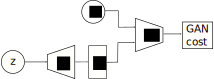
\includegraphics[width=\textwidth]{ambiantgan.pdf}
		\caption{AmbientGAN}
		\label{fig:ambientgan}
	\end{subfigure}
	\hspace{3mm}
	\begin{subfigure}[b]{0.45\textwidth}
		\includegraphics[width=\textwidth]{approach.pdf}
		\caption{Our approach}
		\label{fig:ourapproach}
	\end{subfigure}
	\caption{Different GAN Setups. G and D are the generator and discriminator networks, x and z are samples from the distributions $P_x$ and $P_r$, y is a label/constraint map sampled from $P_y$ and $f_\theta$ is an image degradation function.}
	\label{fig:gansetup}
\end{figure}


\section{Conditional generation as a Maximum A  Posteriori estimation}

Let introduce the formal formulation of the addressed problem. Assume $y$ is the given set of constrained pixel values. To ease the presentation, let consider $y$ as a $n\times p\times c$ image with only a few available pixels (less than $1\%$ of $n\times p\times c$). We will also encode the spatial location of these pixels using a corresponding binary mask $M(y) \in \{0,1 \}^{n\times p\times c}$.  We intend to learn a GAN whose generation network takes as input the constraint map $y$ and the sampled latent code $z \in \setZ$ and outputs a realistic image that fulfills the prescribed pixel values. Within this setup, the generative model can sample from the unknown distribution $p_X$ of the training images $\{x_1, \cdots, x_N\}$ while satisfying unseen pixel-wise constraints at training stage. Formally our proposed GAN can be formulated as
%
\begin{eqnarray}
\label{eq:formulation_our_primary_GAN}
\min_G \max_D L(D,G){\small=}\mathop{\mathbb{E}}_{\substack{x\sim p_{x}}} \Big[\log(D(x))\Big]{\small+} \mathop{\mathbb{E}}_{\substack{z{\small\sim} p_Z\\y{\small\sim} p_{Y}}} \Big[ \log(1{\small -}D(G(y, z)))\Big] \enspace,  \\
\text{s.t. } y = M(y) \odot G(y,z) \nonumber
\end{eqnarray}

\noindent where $\odot$ stands for the Hadamard (or point-wise) product and $M(y)$ for the mask, a sparse matrix with entries equal to one at constrained pixels location. 

As the equality constraint in  Problem (\ref{eq:formulation_our_primary_GAN}) is difficult to enforce during training, we rather investigate a relaxed version of the problems.
%
%A first way to do that is to use the aforementioned CGAN\citep{mirza2014} method, however we focused on using a regularization-based approach.
%To justify our choice of a regularization term, we assume that the errors on the constraints $\epsilon$ follow some common distribution. We then formulate the reconstruction of the constraints as,
%\begin{equation}
%   y = f(G(y, z)) + \epsilon \enspace.
%\label{eq:noisy_generation_primary_CGAN}
%\end{equation}
%
Following Pajot et al. \citep{Pajot2018} we assume that the constraint map is obtained through a noisy measurement process
\begin{equation}
y = f_M(x) + \varepsilon \enspace.
\label{eq:noisy_generation_primary_CGAN}
\end{equation}
Here $f_M$ is the masking operator yielding to $y = M(y) \odot x$. Also the constrained pixels are randomly and independently selected. $\varepsilon$ represents an additive i.i.d noise corrupting the pixels. Therefore
we can formulate the Maximum A Posteriori (MAP) estimation problem, which, given the constraint map $y$, consists in finding the most probable image $x^*$ following the posterior distribution $p_{X|Y}$,
\begin{align}
x^* &= \arg\max_x\log {p_{X|Y}}(x|y) \\
&= \arg\max_x\log p_{Y|X}(y|x) + \log p_X(x) \enspace.
\label{eq:bayesian_formulation_our_primary_CGAN}
\end{align}

\noindent $p_{Y|X}(y|x)$ is the likelihood that the constrained pixels $y$ are issued from image $x$ while $p_X(x)$ represents the prior probability at $x$. Assuming that the generation network $G$ may sample the most probable image $G(y, z)$ complying with the given pixel values $y$, we get the following problem

\begin{equation}
G^* = \arg\max_G \mathop{\mathbb{E}}_{\substack{y\sim p_Y\\z\sim p_Z}} \log {p_{Y|X}}(y|G(y, z)
) + \log p_X(G(y, z)) \enspace.
\label{eq:bayesian_formulation_our_primary_CGAN_G}
\end{equation}

\noindent The first term in Problem (\ref{eq:bayesian_formulation_our_primary_CGAN_G}) measures the likelihood of the constraints given a generated image. Let rewrite Equation (\ref{eq:noisy_generation_primary_CGAN}) as $\vect(y) = \vect(f_M(x)) + \vect(\varepsilon)$ where $\vect(\cdot)$ is the vectorisation operator that consists in stacking the constrained pixels. Therefore, assuming $\vect(\varepsilon)$ is an i.i.d Gaussian noise with distribution $\mathcal{N}(0,\sigma^2 I)$, we achieve the expression of the conditional likelihood
\begin{equation}
log {p_{Y|X}}(y|G(y, z)) \, \propto - \left \|\vect(y) - \vect(M(y) \odot G(y,z))\right\|_2^2 \enspace
\end{equation}
\noindent which evaluates the quadratic distance between the conditioning pixels and their predictions by $G$. In other words, using a matrix notation of  (\ref{eq:noisy_generation_primary_CGAN}), the likelihood of the constraints given a generated image equivalently writes

\begin{equation}
\log {p_{Y|X}}(y|G(y, z) \, \propto - \left \|y - M(y) \odot G(y,z)\right\|_F^2 \enspace.
\end{equation}

\noindent $\| A \|_F^2 $ represents the squared Frobenius norm of matrix $A$ that is the sum of its squared entries. 
%
%In this work, we assume that $\epsilon$ follows a normal distribution $\epsilon\sim\mathcal{N}[0,\sigma^2]$, but it is worth noting that any prior distribution with a close-form solution for maximum likelihood estimation (typically distribution from the exponential family) can be used.
%In the case of the normal distribution, we can minimize our error term by using the $L_2$ norm on the constrained pixels.
%    

The second term in Problem (\ref{eq:bayesian_formulation_our_primary_CGAN_G}) is the likelihood of the generated image under the true but unknown data distribution $p_X$. Maximizing this term can be equivalently achieved by minimizing the distance between $p_X$ and the marginal distribution of the generated samples $G(y,z)$. This amounts to minimizing with respect to $G$, the GAN-like objective function $\mathop{\mathbb{E}}_{\substack{x\sim p_X}} \log(D(x)) + \mathop{\mathbb{E}}_{\substack{z\sim p_Z\\y\sim p_Y}} \log(1-D(G(y, z)))$  \citep{Goodfellow2014}. Putting altogether these elements, we can propose a relaxation of the hard constraint optimization problem (\ref{eq:formulation_our_primary_GAN}) (Figure \ref{fig:ourapproach}) as follows
%minimizing the Jensen-Shannon divergence between the real data distribution and the distribution of the generated data \citep{Goodfellow2014}.

%In our approach, we explicitly model the relaxation of the constraint by minimizing the $L_2$ norm between the constrained pixels and the generated values (see Fig.\ref{fig:ourapproach}).

%The objective function, with $\lambda \geq 0$ an additional parameter, becomes:
\begin{eqnarray}
\min_G \max_D L(D,G) & {\small=} & \mathop{\mathbb{E}}_{\substack{x\sim p_X}} \Big[\log(D(x))\Big] \label{eq:final_optim_problem} \\
&+&\mathop{\mathbb{E}}_{\substack{z\sim p_Z\\y\sim p_Y}} \Big[\log(1-D(G(y, z)))+\lambda \left\|y - M(y) \odot G(y,z)\right\|_F^2 \Big] \enspace . \nonumber
\end{eqnarray}

\subsubsection*{Remarks:}
\begin{itemize}
	\item The assumption of Gaussian noise measurement leads us to explicitly turn the pixel value constraints into the  minimization of the $\ell_2$ norm between the real enforced pixel values and their generated counterparts (see Figure \ref{fig:ourapproach}).
	
	\item This additional term acts as a regularization over prescribed pixels by the mask $M(y)$. The trade-off between the distribution matching loss and the constraint enforcement is assessed by the regularization parameter $\lambda \geq 0$.
	
	\item It is worth noting that the noise $\varepsilon$ can be of any other distribution, according to the prior information, one may associate to the measurement process. We only require this distribution to admit a closed-form solution for the maximum likelihood estimation for optimization purpose. Typical choices are distributions from the exponential family \citep{Brown1986}.
	
\end{itemize}
\begin{figure}[t]
	\centering
	\begin{subfigure}[t]{0.25\textwidth}
		\centering
		\includegraphics[scale=1.5]{origin.png}
		\caption{Original\\Image}
		\label{fig:original_shoe}
	\end{subfigure}\begin{subfigure}[t]{0.25\textwidth}
		\centering
		\includegraphics[scale=1.5]{consts.png}
		\caption{Constraints}
		\label{fig:constraints}
	\end{subfigure}\begin{subfigure}[t]{0.25\textwidth}
		\centering
		\includegraphics[scale=1.5]{img.png}
		\caption{Generated\\Image}
		\label{fig:pixelwise}
	\end{subfigure}\begin{subfigure}[t]{0.24\textwidth}
		\centering
		\includegraphics[scale=1.5]{imgcolor.png}
		\caption{Satisfied\\Consts.}
		\label{fig:generated}
	\end{subfigure}
	\caption[Generation of a sample during training]{Generation of a sample during training. We first sample an image from a training set (\ref{fig:original_shoe}) and we sample the constraints (\ref{fig:constraints}) from it. Then our GAN generates a sample (\ref{fig:pixelwise}). The constraints with squared error smaller than $\epsilon=0.1$ are deemed satisfied and shown by green pixels in (\ref{fig:generated}) while the red pixels are unsatisfied.}
	\label{fig:image_completion}
\end{figure}



To solve Problem (\ref{eq:final_optim_problem}), we use the stochastic gradient descent method. The overall training procedure is detailed in Algorithm \ref{alg:train} and ends up when a maximal number of training epochs is attained. 

When implementing this training procedure we experienced, at inference stage, a lack of diversity in the generated samples (see Figure \ref{fig:diversity_loss}) with deeper architectures, most notably the encoder-decoder architectures. This issue manifests itself through the fact that the learned generation network, given a constraint map $y$, outputs almost deterministic image  regardless the variations in the input $z$. The issue was also pointed out by Yang et al. \citep{Yang2018} as characteristic of CGANs.



\begin{algorithm}[!ht]
	\caption{Proposed training algorithm}
	\label{alg:train}
	\begin{algorithmic}[H]
		\REQUIRE{ $\trainsetX$ the set of  unaltered images, $\trainsetY$ the set of constraint maps, $G$ the generation network, and $D$ the discrimination function}
		\REPEAT
		\STATE sample a mini-batch $\lbrace x_i \rbrace_{i=1}^m$ from $\trainsetX$\;
		\STATE sample a mini-batch $\lbrace y_i \rbrace_{i=1}^m$ from $\trainsetY$\;
		\STATE sample a mini-batch $\lbrace z_i \rbrace_{i=1}^m$ from distribution $p_Z$ \;
		\STATE update $D$ by stochastic gradient ascent of
		\STATE \ \ \ \ $ \sum_{i=1}^{m}\log(D(x_i)) + \log(1-D(G(y_i, z_i)))$
		\STATE sample a mini-batch $\lbrace y_j \rbrace_{j=1}^n$ from $\trainsetY$\;
		\STATE sample a a mini-batch $\lbrace z_j \rbrace_{j=1}^n$ from distribution $p_Z$\;; 
		\STATE update $G$ by stochastic gradient descent of
		\STATE \ \ \ \ $ \sum_{j=1}^n \log(1-D(G(y_j, z_j))) + ||y_j - M(y_j)\odot G(y_j, z_j)||_F^2$\;
		\UNTIL a stopping condition is met
		
	\end{algorithmic}
\end{algorithm}

To avoid the problem, we exploit the recent PacGAN \citep{Lin2018} technique: it consists in passing a set of samples to the discrimination function instead of a single one.  PacGAN is intended to tackle the mode collapse problem in GAN training. The underlying principle being that if a set of images are sampled from the same training set, they are very likely to be completely different, whereas if the generator experiences mode collapse, generated images are likely to be similar.
In practice, we only give two samples to the discriminator, which is sufficient to overcome the loss of diversity as  suggested in \citep{Lin2018}. 
%
The resulting training procedure is summarized in Algorithm~\ref{alg:trainpac}.

\begin{algorithm}[!ht]
	\caption{Our training algorithm including PacGAN}
	\label{alg:trainpac}
	\begin{algorithmic}[H]
		\REQUIRE { $\trainsetX$ the set of  unaltered images, $\trainsetY$ the set of constraint maps, $G$ the generation network, and $D$ the discrimination function}
		\REPEAT
		\STATE sample two mini-batches $\lbrace x_i^a \rbrace_{i=1}^m$, $\lbrace x_i^b\rbrace_{i=1}^m$ from $\trainsetX$\;
		\STATE sample a mini-batch $\lbrace y_i \rbrace_{i=1}^m$ from $\trainsetY$\;
		\STATE sample two mini-batches $\lbrace z_i^a \rbrace_{i=1}^m$, $\lbrace z_i^b \rbrace_{i=1}^m$ from distribution $p_Z$ \;
		\STATE update $D$ by stochastic gradient ascent of
		\STATE \ \ \ \ $ \sum_{i=1}^{m}\log(D(x_i^a, x_i^b)) + \log(1-D(G(y_i, z_i^a), G(y_i, z_i^b)))$
		\STATE sample a mini-batch $\lbrace y_j \rbrace_{j=1}^n$ from $\trainsetY$\;
		\STATE sample two mini-batches $\lbrace z_i^a \rbrace_{i=1}^m$, $\lbrace z_i^b \rbrace_{i=1}^m$ from distribution $p_Z$ \;
		\STATE update $G$ by stochastic gradient descent of
		\STATE \ \ \ \ $ \sum_{j=1}^n \log(1-D(G(y_j, z_j))) + ||y_j - M(y_j)\odot G(y_j, z_j)||_F^2$\;
		\UNTIL a stopping condition is met
		
	\end{algorithmic}
\end{algorithm}







\FloatBarrier

\section{Experiments} \label{sec:experiments_protocol}
We have conducted a series of empirical evaluation to assess the performances of the proposed GAN. Used datasets, evaluation protocol and the tested deep architectures are detailed in this section while Section \ref{sec:results} is devoted to the results presentation. 
\subsection{Datasets}

We tested our approach on several datasets listed hereafter. Detailed  information on these datasets are provided  in the Appendix \ref{app:det_datasets}.
%namely FashionMNIST \citep{Xiao2017}, CIFAR10 \citep{Krizhevsky2009CIFAR10}, CelebA\citep{liu2015celeba} and a custom-made Texture texture dataset:
\begin{description}
	\item{FashionMNIST} \citep{Xiao2017} consists of 60,000 $28\times 28$ small grayscale images of fashion items, split in 10 classes and is a harder version of the classical MNIST  dataset \citep{LeCun1998a}. %known to be simple to solve. 
	The very small size of the images makes them particularly appropriate for large-scale experiments, such as hyper-parameter tuning. 
	
	\item{CIFAR10} \citep{Krizhevsky2009} consists of 60,000 $32 \times 32$ colour images of 10 different and varied classes. It is deemed less easy than MNIST and FashionMnist
	%considered harder to learn that MNIST and FashionMNIST, even it is of nearly the same dimension.
	\item{CelebA}\citep{Liu2015} is a large dataset of celebrity portraits labeled by identity and a variety of binary features such as eyeglasses, smiling... We use 100,000 images cropped to a size of $128 \times 128$, making this dataset appropriate for a high dimension evaluation of our approach in comparison with related work.
	
	\item{Texture} is a custom dataset 
	%was eventually created that is composed of texture, sampling $20000$ patches
	composed of $20,000$ $160 \times 160$ patches sampled from a large brick wall texture, as recommended in \citep{Jetchev2016texture}. It is worth noting that this procedure can be reproduced on any texture image of sufficient size. Texture is a testbed of our approach on fully-convolutional networks for constrained texture generation task. 
	%This allows us to experiment fully-convolutional architectures on a texture reconstruction task.
	
	\item{Subsurface} is a classical dataset in geological simulation \citep{Strebelle2002} which consists, similarly to the Texture dataset, of 20,000  $160 \times 160$ patches sampled from a model of a subsurface binary domain. These models are assumed to have the same properties as a texture, mainly the property of global ergodicity of the data.
\end{description}

To avoid learning explicit pairing of real images seen by the discrimination function with constraint maps provided to the generative network, we split each dataset into training, validation and test sets, to which we add a set composed of constraint maps that should remain unrelated to the three others.
In order to do so, a fifth of each set is used to generate the constrained pixel map $y$ by randomly selecting $0.5\%$ of the pixels from a uniform distribution, composing a set of constraints for each of the train, test and validation sets. The images from which these maps are sampled are then removed from the training, testing and validation sets. For each carried experiment the best model is selected based on some performance measures (see Section \ref{subs:eval}) computed on the validation set. Finally, reported results are computed on the test set.

%To avoid learning explicit correlations between real examples presented to the discriminator and constraint maps given to the generator, we create a splitting consisting in the classical train, validation and test databases, to which we add a constraints database that should remain unrelated to the three others. A fifth of each set is used to generated the matrix of constraints $C$ by randomly selecting $0.5\%$ of the pixels, uniformly. These images are then removed from the training, testing and validation sets.


\subsection{Network architectures}
\label{subs:architectures}

We use a variety of GAN architectures in order to adapt to the different scales and image sizes of our datasets. The detailed configuration of these architectures are exposed in Appendix \ref{app:det_archis}.

For the experiments on the FashionMNIST \citep{Xiao2017}, we use a lightweight network for both the discriminator and the generator similarly to DCGAN  \citep{Radford2015} due to the small resolution of FashionMnist images.
%This is motivated by the large number of experiments and the small dimension of the images.

To experiment on the Texture dataset, we consider a set of fully-convolutional generator architectures based on either dilated convolutions \citep{Yu2015}, which behave well on texture datasets \citep{Ruffino2019}, or encoder-decoder architectures that are commonly used in domain-transfer applications such as CycleGAN \citep{Zhu2017}. We selected these architectures because they have very large receptive fields without using pooling, which allow the generator to use a large context for each pixel.

We keep the same discriminator across all the experiments with these architectures, the PatchGAN discriminator \citep{Isola2016}, which is a five-layer fully-convolutional network with a sigmoid activation.

The Up-Dil architecture consists in a set of transposed convolutions (the upscaling part), and a set of dilated convolutional layers \citep{Yu2015}, while the Up-EncDec has an upscaling part followed by an encoder-decoder section with skip-connections, where the constraints are downscaled, concatenated to the noise, and re-upscaled to the output size.

The UNet \citep{Ronneberger2015} architecture is an encoder-decoder where skip-connections are added between the encoder and the decoder.
The Res architecture is an encoder-decoder where residual blocks \citep{He2015} are added after the noise is concatenated to the features. The UNet-Res combines the UNet and the Res architectures by including both residual blocks and skip-connections.

Finally, we will evaluate our approach on the Subsurface dataset using the architecture that yields to the best performances on the Texture dataset.
%
\subsection{Evaluation}
\label{subs:eval}
We evaluate our approach based on both the satisfaction of the pixel constraints and the visual quality of sampled images. From the assumption of Gaussian measurement noise (as discussed in Section \ref{sec:our-approach}), we assess the constraint fulfillment using the following mean square error (MSE) 
\begin{equation}
MSE = \frac{1}{L} \sum_{i=1}^L \left\|y_i - M(y_i) \odot G(y_i, z_i)\right\|_F^2
\end{equation}
This metric should be understood as the mean squared error of reconstructing the constrained pixel values. 

%On one hand, we simply use the mean squared error between the provided constrained values and the constrained pixels in the generated image to evaluate the respect of the constraints.
%On the other hand, 
Visual quality evaluation of an image is not a trivial task \citep{Theis2015}. However, Fréchet Inception Distance (FID) \citep{Heusel2017} and Inception Score \citep{Salimans2016}, have been used to evaluate the performance of generative models. We employ FID since the Inception Score has been shown to be less reliable \citep{Barratt2018}. The FID consists in computing a distance between the distributions of relevant features extracted from generated and real samples. To extract these features, a pre-trained Inception v3 \citep{Szegedy2016} classifier is used to compute the embeddings of the images  at a chosen layer. Assuming these embeddings shall follow a normal distribution, the quality of the generated images is assessed in term of a Wasserstein-2 distance between the distribution of real samples and generated ones. Hence the FID writes
%
%It then assumes that these features are normal, and compare the (normal) distributions of the features from the real data and the fake ones using a Fréchet (or Wasserstein-2) distance, 

\begin{equation}
FID = ||\mu_r - \mu_g||^2+Tr(\Sigma_r+\Sigma_g - 2(\Sigma_r\Sigma_g)^{1/2}),
\label{eq:fid}
\end{equation}

\noindent where $Tr$ is the trace operator, ($\mu_r$, $\Sigma_r$) and ($\mu_g$, $\Sigma_g$) are the pairs of mean vector and covariance matrice of embeddings obtained on respectively the real and the generated data. Being a distance between distributions,  a small FID corresponds to a good matching of the distributions.
%corresponds to a , better the distr

Since the FID requires a pre-trained classifier adapted to the dataset in study, we trained simple convolutional neural networks as classifiers for the FashionMNIST and the CIFAR-10 datasets. For the Texture dataset, since the dataset is not labeled, we resort to a CNN classifier trained on the Describable Textures Dataset (DTD) \citep{Cimpoi14}, which is a related application domain.

However, since we do not have labels for the Subsurface dataset, we could not train a classifier for this dataset, thus we cannot compute the FID. To evaluate the quality of the generated samples, we use metrics based on a distance between feature descriptors extracted from real samples and generated ones. Similarly to \citep{Ruffino2019}, we rely on a $\chi^2$ distance between the Histograms of Oriented Gradients (HOG) or Local Binary Patterns (LBP) features computed on generated and real images. 

Histograms of Oriented Gradients (HOG) \citep{Dalal2005} and Local Binary Patterns (LBP) \citep{Pietikainen2011a} are computed by splitting an image into cells of a given radius and computing on each cell the histograms of the oriented gradients for HOGs and of the light level differences for each pixel to the center of the cell for LBPs.  Additionally, we consider the domain-specific metric, the connectivity function \citep{Lemmens2017} which is presented in Appendix \ref{app:geostatistics}.

Finally, we check by visual inspection if the trained model $G$ is able to generate diverse samples, meaning that for a given $y$ and for a set of latent codes $(z_1, ..., z_n) \sim p_Z$, the generated samples $G(y,z_1), \ldots, G(y, z_n)$ are visually different. 

%Since we empirically observed that our models were either producing very different samples or samples that only differ by a small noise factor, we do not propose a specific evaluation metric and instead check manually if a loss of diversity occurs.



\section{Experimental evaluation and application to underground soil generation}

\subsection{Quality-fidelity trade-off}

% \begin{figure}[!]
%     \centering
%     \includegraphics[trim=0 0 0 40, clip,scale=0.35]{MSE_mnist}\includegraphics[trim=0 0 0 40, clip,scale=0.35]{MSE_fashion}
%     \includegraphics[trim=0 0 0 40, clip,scale=0.35]{FID_mnist}\includegraphics[trim=0 0 0 40, clip,scale=0.35]{FID_fashion}

%     \centering
%     \caption{MSE (top) and  FID (bottom) w.r.t. the regularization parameter $\lambda$;
%     Dataset MNIST (left), Fashion MNIST (right).
%     %The different orders of magnitude for the Y-axis of the FID is due to the different classifiers used to compute this distances.
%     }
%     \label{fig:fids}
%     \label{fig:mses}
% \end{figure}

\begin{figure}[t]
	\centering
	\includegraphics[trim=0 0 0 40, clip,scale=0.4]{MSE_fashion}\includegraphics[trim=0 0 0 40, clip,scale=0.4]{FID_fashion}
	
	\includegraphics[scale=0.5]{pareto_fashion}
	
	\centering
	\caption{Our approach compared to the GAN and CGAN baselines. MSE (left) and  FID (right) w.r.t. the regularization parameter $\lambda$, MSE w.r.t the FID (bottom).
		%The different orders of magnitude for the Y-axis of the FID is due to the different classifiers used to compute this distances.
	}
	\label{fig:fids}
	\label{fig:mses}
	\label{fig:paretos}
\end{figure}

%In this set of experiments, 
We first study the influence of the $\lambda$ regularization hyper-parameter on both the quality of the generated samples and the respect of the constraints. We experiment on the %MNIST \citep{Lecun1998} and
FashionMNIST \citep{Xiao2017} dataset, since such a study requires intensive simulations permitted by the low resolution of FashionMnist images and the used architectures (see Section \ref{subs:architectures}). 
%a lot of re-training and the small size of the images allowed us to run several hundreds of experiments.

To overcome classical GANs instability, the networks are trained 10 times and the median values of the best scores on the test set at the best epoch 
are recorded. The epoch that minimizes:
\begin{equation*}
\sqrt{\left(\frac{FID - FID_{min}}{FID_{max}- FID_{min}}\right)^2 + \left(\frac{MSE - MSE_{min}}{MSE_{max}- MSE_{min}}\right)^2}
\end{equation*}  on the validation set is considered as the best epoch, where $FID_{min}$, $MSE_{min}$, $FID_{max}$ and $MSE_{max}$ are respectively the lowest and highest FIDs and MSEs obtained on the validation set.

Empirical evidences (highlighted in Figure \ref{fig:mses}) show that with a good choice of $\lambda$, the regularization term helps the generator to enforce the constraints, leading to smaller MSEs than when using the CGAN ($\lambda=0$) without compromising on the quality of generated images. Also, we can note that using the regularization term even leads to a better image quality compared to GAN and CGAN.
%
The bottom panel in Figure \ref{fig:paretos} illustrates that the trade-off between image quality and the satisfaction of the constraints can be controlled by appropriately setting the value of $\lambda$. Nevertheless, for small values of $\lambda$ (less or equal to $10^{-1}$), our GAN model fails to learn meaningful distribution of the training images and only generates uniformly black images. This leads to the plateaus on the MSE and FID plots (top panels in Figure \ref{fig:mses}).


% \begin{figure}
%     \centering
%     \includegraphics[trim=0 0 0 40, clip,scale=0.4]{pareto_mnist}\includegraphics[trim=0 0 0 40, clip,scale=0.4]{pareto_fashion}
%     \vspace*{-3mm}
%     \caption{MSE w.r.t the FID. Left: MNIST; Right: Fashion MNIST. Note that due to the failure mode previously mentioned, a large part of the values are stacked in the top right corner of these figures.
%     }
%     \label{fig:paretos}
% \end{figure}  

\subsection{Texture generation with fully-convolutional architectures}
\label{sub:fcnn}
Fully-convolutional architectures for GANs are widely used, either for domain-transfer applications \citep{Zhu2017}\citep{Isola2017} or for texture generation \citep{Jetchev2016}. In order to evaluate the efficiency of our method on relatively high resolution images, we experiment the fully-convolutional networks described in Section \ref{subs:architectures} on a texture generation task using Texture dataset. We investigate the upscaling-dilatation network, the encoder-decoder one and the resnet-like architectures.

Our training algorithm was run for 40 epochs on all reported results. We provide a comparison to CGAN\citep{Mirza2014} approach by using the selected best architectures.
The models are evaluated in terms of best FID (visual quality of sampled images) at each epoch and MSE (conditioning on fixed pixel values).  We also compute the FID score of the models at the epochs where the MSE is the lowest. In the other way around, the MSE is reported at epoch when the FID is the lowest. The obtained quantitative results are detailed in Table \ref{tab:ablation}.

For the encoder-decoder models, we can notice that the models using ResNet blocks perform better than just using a UNet generator. A trade-off can also be seen between the FID and MSE for the ResNet models and the UNet-ResNet, which could mean that skip-connections help the generator to fulfill the constraints but at the price of lowered visual quality.

Although the encoder-decoder models perform the best, they tend to lose diversity in the generated samples (see Figure \ref{fig:diversity_loss}), whereas the upscaling-based models have high FID and MSE but naturally preserve diversity in the generated samples.

\begin{figure}
	\centering
	\includegraphics[width=2cm]{diversity_1.png}\hspace{0.5cm}\includegraphics[width=2cm]{diversity_2.png}\hspace{0.5cm}\includegraphics[width=2cm]{diversity_1_pac.png}\hspace{0.5cm}\includegraphics[width=2cm]{diversity_2_pac.png}
	
	\vspace{0.3cm}
	\includegraphics[height=4cm]{diversity_diff_nobar.png}\hspace{0.5cm}\includegraphics[height=4cm]{diversity_diff_pac.png}
	\caption{An example of a loss of diversity when generating Texture samples with a trained UNetRes network using two different random noises $z$ and a single constraint map $y$. The two samples on the top left are generated using the classical GAN discriminator whereas the samples on the top right are generated using the PacGAN approach. The loss of diversity is clearly visible on the absolute differences between the greyscaled images (bottom).}
	\label{fig:diversity_loss}
\end{figure}

Changing the discriminator for a PacGAN discriminator with 2 samples in the encoder-decoder based architectures allows to restore diversity, while keeping the same performances as previously or even increasing the performances for the UNetRes (see Table \ref{tab:ablation}).

Table \ref{tab:ablation-cgan} compares our proposed approach to CGAN using fully convolutional networks. It shows that our approach is more able to comply with the pixel constraints while producing realistic images. Indeed, our approach outperforms CGAN (see Table \ref{tab:ablation-cgan}) by a large margin on the respect of conditioning pixels (see the achieved MSE metrics by  our UNetPAC or UNetResPAC)  and gets  close FID performance on the generated samples. This finding is in accordance of the obtained results on FashionMnist experiments.
%show that the comparison with the CGAN approach still holds well in a fully-convolutional setting since our approach outperforms CGAN by a large margin on the respect of the constraints and come close to it on the visual quality of the generated samples. This conforms the results obtained on the previous experiments on the FashionMNIST dataset.

\begin{table}
	\centering
	\begin{tabular}{|l|c|c|c|c|c|}
		\hline
		Model           & Best FID & Best MSE & FID at & MSE at & Diversity\\
		&&&best MSE & best FID & \\
		\hline
		Up-Dil      & 0.0949 & 0.4137 & 1.0360 & 0.7057 & {\color{green}\cmark } \\
		Up-EncDec  & 0.1509 & 0.7570 & 0.2498 & 0.9809 & {\color{green}\cmark } \\
		UNet        & 0.0442 & 0.1789 & 0.0964 & 0.4559 & {\color{red}\xmark } \\
		Res      & 0.0458 & 0.0474 & 0.0590 & 0.0476 & {\color{red}\xmark } \\
		UNetRes & 0.0382 & 0.0307 & 0.0499 & 0.0338 & {\color{red}\xmark } \\
		\hline
		ResPAC &  \textbf{0.0350} & 0.0698 & 0.0466 & 0.4896 & {\color{green}\cmark } \\
		UNetPAC &  0.0672 & \textbf{$\leq$ 0.0001} & 0.3120 & 0.2171&  {\color{green}\cmark } \\
		UNetResPAC & 0.0431 & 0.0277 & \textbf{0.0447} & \textbf{0.0302} &  {\color{green}\cmark }\\
		\hline
	\end{tabular}
	
	\caption{Results obtained by the different fully-convolutional architectures on the Texture dataset. We can remark that the encoder-decoder greatly outperforms the upscaling ones and that using the PacGAN technique helps keeping the performance of these models while restoring the diversity in the samples. The bottom part of the table refers to PacGan architectures.}
	\label{tab:ablation}
\end{table}

\begin{table}[t]
	\centering
	\begin{tabular}{|l|c|c|c|c|c|}
		\hline
		Model           & Best FID & Best MSE & FID at & MSE at \\
		&&&best MSE & best FID  \\
		\hline
		CGAN-ResPAC &   \textbf{0.0234} & 0.1337 &  \textbf{0.0340} & 0.2951 \\
		CGAN-UNetPAC &  0.0518 & 0.2010 & 0.0705 & 0.4828\\
		CGAN-UNetResPAC & 0.0428 & 0.1060 & 0.0586 & 0.2250\\
		\hline
		Ours-ResPAC &  0.0350 & 0.0698 & 0.0466 & 0.4896\\
		Ours-UNetPAC &  0.0672 & \textbf{$\leq$ 0.0001}  & 0.3120 & 0.2171 \\
		Ours-UNetResPAC & 0.0431 & 0.0277 &0.0447 & \textbf{0.0302}\\
		\hline
	\end{tabular}
	
	\caption{Results obtained by the selected best fully-convolutional architectures on the Texture dataset for both the CGAN approach and our approach.}
	\label{tab:ablation-cgan}
\end{table}

\subsection{Extended architectures}
We extend the comparison of our approach to CGAN on the CIFAR10 and CelebA  datasets (Table \ref{tab:cifar10}). We investigated the architectures described in Section \ref{subs:architectures}. All reported results are obtained with the regularization parameter fixed to $\lambda=1$.
We train the networks for 150 epochs using the same dataset split as stated previously in order to keep independence between the images constraint maps. The evaluation procedure remains also unchanged. We use the PacGAN approach to avoid the loss of diversity issues. The experiments on both datasets show that though CGAN  provides better results in terms of visual quality, our approach outperforms it according to the respect of the pixel constraints.


\begin{table}
	\centering
	\begin{tabular}{|l|c|c|c|c|c|}
		\hline
		&Model           & Best FID & Best MSE & FID at & MSE at \\
		&&&&best MSE & best FID \\
		\hline
		CIFAR-10 &CGAN   & \textbf{2,68}  & 0.081  & \textbf{2.68}  & 0.081\\
		&Ours            & 3.120 & \textbf{0.010} & 3.530 & \textbf{0.011} \\    
		\hline
		CelebA &CGAN      & \textbf{1.34e-4} & 0.0209 &  \textbf{1.81e-4} & 0.0450\\
		&Ours            & 2.09e-4& \textbf{0.0053} & 5.392e-4 & \textbf{0.0249} \\
		\hline
	\end{tabular}
	
	\caption{Results on the CIFAR10 and CelebA datasets. The reported performances compare CGAN to our proposed GAN conditioned on scarce constraint map.}
	\label{tab:cifar10}
\end{table}

\vspace{0.4cm}

\subsection{Application to hydro-geology}

Finally, we evaluate our approach on the Subsurface dataset. We use the UNetResPAC  architecture, since it performed the best on Texture data as exposed in Section \ref{sub:fcnn}. As previously, we simply set the regularization parameter at $\lambda=1$ and, the network is trained for 40 epochs using the same experimental protocol. To evaluate the trade-off between the visual quality and the respect of the constraints, instead of FID we rather compute distances between visual Histograms of Oriented Gradients (see Section \ref{sec:experiments_protocol}), extracted from real and generated samples. We also evaluate the visual quality of our approach with a distance between Local Binary Patterns. Indeed, Subsurface application lacks labelled data in order to learn a deep network classifier from which the FID score can be computed. 

%As stated before in Section \ref{subs:eval}, we cannot use the FID to evaluate the visual quality of the generated images since we don't have a supervised task linked to the data.
%Therefore we use distances between visual features, namely Histograms of Oriented Gradients and Local Binary Patterns (see Section \ref{sec:experiments_protocol}), extracted from real and generated samples.

The obtained results are summarized in Tables \ref{tab:subsurface} and \ref{tab:subsurface_visual}. They are coherent with the previous experiments since the generated samples are diverse and have a low error regarding the constrained pixels. The conditioning have a limited impact on the visual quality of the generated samples and compares well to unconditional approaches \citep{Ruffino2018}. Evaluation of the generated images using the domain-connectivity function highlights this fact on Figures \ref{fig:ours_connectivity} and \ref{fig:ours_connectivity} in the supplementary materials. Also examples of generated images by our approach  pictured in Figure \ref{fig:samples_subsurface} (see appendix \ref{app:generated_images}) show that we preserve the visual quality and honor the constraints.

\begin{table}
	\centering
	\begin{tabular}{|l|c|c|c|c|c|}
		\hline
		&Model           & Best HOG & Best MSE& HOG at & MSE at \\
		&&& &  best MSE & best HOG \\
		\hline
		Subsurface &CGAN   & \textbf{2.92e-4} & 0.2505 & \textbf{3.06e-4}  & 1.1550 \\
		&Ours            & 4.31e-4 & \textbf{0.0325}& 5.69e-4 & \textbf{0.2853} \\
		\hline
	\end{tabular}
	\caption{Evaluation of the trade-off between the visual quality of the generated samples and the respect of the constraints for the CGAN approach and ours on the Subsurface dataset.}
	\label{tab:subsurface}
\end{table}

\begin{table}[h]
	\centering
	\begin{tabular}{|l|c|c|c|c|c|}
		\hline
		&Model           & Best HOG & Best MSE& Best LBP & Best LBP \\
		&&& & (radius=1) & (radius=2) \\
		\hline
		Subsurface &CGAN   & \textbf{2.92e-4} & 0.2505 & \textbf{2.157} & \textbf{3.494}\\
		&Ours            &  4.31e-4 &\textbf{0.0325} & 10.142 & 16.754 \\
		\hline
	\end{tabular}
	\caption{Evaluation of the visual quality between the CGAN approach and ours on the Subsurface dataset using several metrics.}
	\label{tab:subsurface_visual}
\end{table}



\section*{Conclusion}
In this paper, we address the task of learning effective generative adversarial networks when only very few pixel values are known beforehand. To solve this pixel-wise conditioned GAN, we model the conditioning information under a probabilistic framework. This leads to the maximization of the likelihood of the constraints given a
generated image. Under the assumption of a Gaussian distribution over the given pixels, we formulate an objective function composed of the conditional GAN loss function regularized by a $\ell_2$-norm on pixel reconstruction errors. We describe the related optimization algorithm.

Empirical evidences illustrate that the proposed framework helps obtaining good image quality while best fulfilling the constraints compared to classical GAN approaches. We show that, if we include the PacGAN technique,  this  approach  is  compatible  with  fully-convolutional  architectures  and scales well to large images. We apply this approach to a common geological simulation task and show that it allows the generation of realistic samples which fulfill the prescribed constraints.

In future work, we plan to investigate other prior distributions for the given pixels as the Laplacian or $\beta$-distribtutions. We are also interested in applying the developed approach to other applications or signals such as audio inpainting \citep{Marafioti2018}.



{\Huge END OF THE COPY PASTED AREA}


 \section{Image Reconstruction, Inpainting and Compressed Sensing}

Image reconstruction is the task of completing an image from a very small subset of the pixels. Such source data can usually be found in domains where the measurement process is very noisy or where measurements are expensive. This task differs from image inpainting since the source data is usually unstructured and very scarce, as in this chapter we will consider randomly scattered measurements of less than a percent of the image. While our discussion focus on image reconstruction, it is noteworthy to mention that this applies to other kinds of signals.

The task of image reconstruction is challenging since very few information is available for use. To overcome this lack of information, generative models such as GANs leverage on existing datasets to learn the distribution of the real images. By conditioning the learned distribution, a GAN could learn to generate an image while enforcing the constraint that the pixels known beforehand must remain similar in the generated image.

Similarly as in the GAN setup, we denote  by $X \in \setX$ a random variable and $x$ its realization. Let $p_X$ be the distribution of $X$ over $\setX$ and $p_X(x)$ be its evaluation at $x$. Similarly $p_{X|Y}$ represents the distribution of $X$ conditioned on the random variable $Y \in \setY$. 

We denote by $x \in \setX = [-1, 1]^{n\times p\times c}$  (see Figure \ref{fig:digit}) an image sampled from an unknown distribution $p_X$  and a sparse matrix  $y \in  \setY = [-1, 1]^{n\times p\times c}$ (Figure \ref{fig:pixelwise_gen}) as the given constrained pixels. The problem  then consists in finding a generative model $G$ with inputs $z$ (a random vector sampled from a known distribution $p_Z$ over the space $\setZ$) and constrained pixel values $y \in  [-1, 1]^{n\times p\times c}$ that maps the distribution $p_Z$ onto the conditional distribution $p_{X|Y}$ of the real images given the constraints $y$ (see Figure \ref{fig:image_completion}).

\begin{figure}[t]
	\centering
	\begin{subfigure}[t]{0.33\textwidth}
		\centering
		\includegraphics[width=3cm]{fashion_sample.jpg}
		\caption{Original \\ Image}
		\label{fig:digit}
	\end{subfigure}\begin{subfigure}[t]{0.33\textwidth}
		\centering
		\includegraphics[width=3cm]{fashion_sample_inpainting.jpg}
		\caption{Inpainting\\Input}
		\label{fig:inpainting}
	\end{subfigure}\begin{subfigure}[t]{0.33\textwidth}
		\centering
		\includegraphics[width=3cm]{fashion_sample_pixel.jpg}
		\caption{Constraint\\Map}
		\label{fig:pixelwise_gen}
	\end{subfigure}
	\caption[The problems of inpainting and image reconstruction]{Difference between regular inpainting (\ref{fig:inpainting}) and the problem undertaken in this work (\ref{fig:pixelwise_gen}) on a real sample (\ref{fig:digit}).}
	\label{fig:image_completion_task}
\end{figure}

\begin{figure}[t]
\centering
\begin{subfigure}[t]{0.25\textwidth}
	\centering
	\includegraphics[scale=1.5]{origin.png}
	\caption{Original\\Image}
	\label{fig:original_shoe}
\end{subfigure}\begin{subfigure}[t]{0.25\textwidth}
	\centering
	\includegraphics[scale=1.5]{consts.png}
	\caption{Constraints}
	\label{fig:constraints}
\end{subfigure}\begin{subfigure}[t]{0.25\textwidth}
	\centering
	\includegraphics[scale=1.5]{img.png}
	\caption{Generated\\Image}
	\label{fig:pixelwise}
\end{subfigure}\begin{subfigure}[t]{0.24\textwidth}
	\centering
	\includegraphics[scale=1.5]{imgcolor.png}
	\caption{Satisfied\\Consts.}
	\label{fig:generated}
\end{subfigure}
\caption[Generation of a sample during training]{Generation of a sample during training. We first sample an image from a training set (\ref{fig:original_shoe}) and we sample the constraints (\ref{fig:constraints}) from it. Then our GAN generates a sample (\ref{fig:pixelwise}). The constraints with squared error smaller than $\epsilon=0.1$ are deemed satisfied and shown by green pixels in (\ref{fig:generated}) while the red pixels are unsatisfied.}
\label{fig:image_completion}
\end{figure}


\CR{
Related works : CGAN, GAN inpainting

Limitations of these models
}

\section{Conditional generation as a Compressed Sensing problem}

Sparsity prior, $\ell_0$ norm minimization, Lasso regularization

Deep image prior

%https://arxiv.org/pdf/1703.03208.pdf

%http://corelab.ntua.gr/ml-seminar/slides/Dimakis_NTUA.pdf
 Compressed Sensing with Meta-Learning
 AmbientGAN, UNIR
 
\section{Conditional generation as a Maximum A  Posteriori estimation}
Approche de l'article NeuCom :

Formulation as a Maximum A Posteriori Estimation, assumptions (normal error)

Construction of the loss term using bayes rule and least squares 

PacGAN for keeping the diversity

\section{Experimental evaluation and application to underground soil generation}

Datasets : MNIST/FashionMNIST/CelebA/Texture

Evaluation : MSE/FID; Epoch  selection criterion

Architectures : Appendix ? DCGAN + SGAN (encoder-decoder)

Results : visible trade-off, good fidelity overall

Application to hydro-geology : subsurface dataset

Evaluation : MSE/HOG+LBP

\section{Conclusion}

Objective reached : tuneable loss, pixel-wise, keeping diversity

Applications in hydro-geology : papier Eric

Future works : other distributions (modelling error using Laplacian, beta or Poisson distributions)

\chapter{Conditioning generation with multiple task-specific constraints}
\label{chap:chapter3}


\begin{chapterabstract}
	The problem addressed in this chapter is the generation of polarimetric images using Cyle-Consistent Generative Adversarial Networks (CycleGAN) with constraints derived from the optics of polarimetry. The conducted research is motivated by the increasing popularity of the combination of deep learning frameworks with polarimetric imaging in various domains, including medical imaging and scene analysis. Even if polarimetric imaging has shown improved performances, their robustness may be questioned because of the small size of the training datasets. 
	This issue could be resolved by data augmentation. However, polarization modality is subject to some physical feasibility constraints that could be impeded with classical data augmentation techniques. In this paper we propose a framework based on CycleGAN, integrating the constraints of polarimetric images during training stage. We evaluate the proposed generative model on road scene images. 
	The obtained results achieved an effective generation of physical polarization-encoded images. Further experiments on the task of road object detection show that with the generated images, the detection of cars and pedestrian are improved by up to 9\%.
\end{chapterabstract}

%===========================================================
\section{Introduction}


Generative  adversarial networks (GAN) \citep{Goodfellow2014,Wang2019} are powerful deep generative models used to  implicitly learn complex data distributions and to generate realistic samples from them. In its standard form, a GAN consists of two models: a generator which maps samples drawn from a latent low-dimensional distribution (usually uniform or gaussian distributions) to  high-dimensional points expected to follow the sought data distribution, and a discrimination model which discriminate the real samples from the generated ones \citep{Goodfellow2014}.  GANs have proven remarkable in various application domains including  image generation \citep{Arjovsky17}, image-to-image translation \citep{Isola2016, Zhu2017, Hoffman18} or image attribute manipulation \citep{Antipov2017} to name a few. 

Arguably most of the impressive achievements of the GAN were obtained for RGB images. A body of work attempted to extend GAN architectures to other uncommon imaging domains. For instance, some existing methods rely on CycleGAN \citep{Zhu2017a}, an image-to-image translation network, to generate infrared road scenes from RGB counterpart images \citep{Zhang2018b}, to produce thermal images for person re-identification \cite{Knia2018} or for infrared image colorization \cite{Mehri2019}. In the same vein,  \citet{Nie2017} achieved data augmentation in the field of medical imaging by transforming MRI inputs into pseudo-CT images.  From another point of view, \citet{Sallab2019} used CycleGANs to produce realistic LiDAR points cloud from simulated ones. 


Following the previous stream of work, this paper contributes generative models for non-conventional imaging techniques. Specifically we propose a  generative model framework to produce realistic polarimetric images.  The significant interest resides in the fact that polarimetric imaging is a rich modality that enables to characterize an object by its reflective properties. Those properties are object specific, hence, they convey strong features to analyse the content of a scene. In a polarimetric image, each pixel encodes information regarding the object's roughness, its orientation and its reflection \citep{Wolff1995}. Applications of polarimetric imaging range from indoor autonomous navigation \citep{Berger2017}, depth map estimation \citep{Zhu2019}, 3D objects reconstruction \citep{Morel2006} to differentiation of healthy and unhealthy cervical tissues in order to detect cancer at an early stage \citep{Rehbinder2016}. Also, recently, polarization imaging was exploited in autonomous driving applications either to enhance car detection \citep{Fan2018}, road mapping and perception \citep{Aycock2017} or to detect road objects in adverse weather conditions \citep{Blin2019}.  However, these  applications are characterized by the reduced size of the available training databases which restrains them from using deep neural networks, thus the need of polarimetric data generation model. 

Contrary to RGB, LiDAR or infrared image generation which mostly responded to visual qualitative  constraints, unless some learnable knowledge constraints are enforced (see \cite{Hu2018} for pose conditional person image generation), sampling polarization images is more challenging. Indeed, this imaging technique comes with physical admissibility constraints on the pixels of an image. To be physically feasible, each pixel entry of such an image should satisfy some physical constraints related to light polarization principle and to the calibration setup of the acquisition devices.
Therefore, we formulate our problem of polarimetric image generation as a CycleGAN learning problem under physical constraints to ensure that the generated images are valid. CycleGANs \citep{Zhu2017a} enabled to achieve unpaired image-to-image translation with only a few number of images. 
They allow to circumvent the expensive labelling step by transferring a source labelled dataset to one or multiple target domain \citep{Almahairi2018} by keeping unchanged the shapes of the source image. 


Starting from unpaired sets of RGB and polarimetric images, we propose a learning framework based on CycleGAN and able to handle the physical polarization constraints during training. We demonstrate the effectiveness of our constrained-output CycleGAN on the KITTI dataset \citep{Geiger2012} and the Berkeley Deep Drive dataset (BDD100K) \cite{Xu2017}, two common datasets used for object detection in road scenes. Using the generated polarization-encoded images to train a deep object detectors, we witness an improvement of the detection performances of cars and pedestrians which are of great interest for autonomous driving applications. 

To summarize, the contributions of this paper are:
\begin{itemize}
	\item as far as our knowledge can go, we propose the first framework for generating physical polarization-encoded images starting from RGB images, 
	\item we propose an extension of CycleGAN which allows to generate polarimetric-encoded images while handling the physical constraints the pixels of the generated image should satisfy,
	\item when plugged into the training procedure of an object detector for pre-training, the generated images help improving the detection performances.
\end{itemize}

The remainder of the paper is organized as follows:  
the polarization formalism and the physical constraints it involves are first presented. Then, the image-to-image translation using Cycle-Consistent GAN is described and a way to take into account these physical constraints during the training process of the CycleGAN for generating polarimetric images is investigated. Experimental evaluations are conducted ; they aim to translate RGB images of KITTI and BDD100K datasets into polarimetric images. Finally, the generated images are exploited to boost the performances of an object detection network. The code for the experiments is available at: \url{https://anonymous.4open.science/r/4a83820e-9c65-417c-af3a-ab2979d6e2e8/}

%%%%%%%%%%%%%%%%%%%%%%%%%%%%%%%%%%%%%%%%%%%%%%%%%%%%%%%%%%%%%%%%%%%%%%%%%%%%%%%%%%%%%%%%%%%%%%%%%%%

\section{Framework}

This section introduces the polarization formalism, the Generative Adversarial Network approach and the CycleGAN principles. It focuses on the formulation of the proposed modelling framework, namely the learning of a CycleGAN with output constraints. A solution approach is detailed and the related learning principle is presented. 

\subsection{Polarization formalism}
\label{physical_prop}

Light waves can oscillate in different orientations. Polarization represents the direction of propagation of the electrical field of the light wave. When the direction is linear, elliptical or circular, the polarization state is said to be totally polarized. However, it is partially polarized or non polarized when the light wave partly propagates in a random way \citep{Bass1995}. 

Polarimetric imaging consists in representing the polarization state of the light wave reflected from each part of the scene. When an unpolarized light wave is being reflected, it becomes partially linearly polarized. Its polarization depends on the normal surface  and the refractive index of the material it impinges on. The linear part of the reflected light can be described by measurable parameters and specifically by the linear Stokes vector $S = \begin{bmatrix}
S_0 & S_1 & S_2 \end{bmatrix}^\top$ where $S_0>0$ represents the total intensity, $S_1$ the amount of horizontally and vertically linearly polarized light and $S_2$ the amount of linearly polarized light at $\pm$~45\degree. 
%
It is important to note that by design, the Stokes vector is physically admissible if and only if the two following conditions are met:  
%
\begin{equation}
S_0 > 0
\quad \mbox{ and } \quad 
S_0^2 \geqslant S_1^2 + S_2^2 \enspace.
\label{eqn:stokes_constraint_S0}
\end{equation}

One salient physical property, obtained from the Stokes parameters, is the degree of polarization (DOP) \citep{Ainouz2013}  defined by:
$$
DOP = \frac{\sqrt{S_1^2+S_2^2}}{S_0} \enspace.
$$
%
The $DOP \in [0,1]$ refers to the amount of polarized light in a wave. It is equal to 1 for a totally polarized light, 0 for unpolarized light and between 0 and 1 for partially polarized light.

Polarization images are accordingly obtained by the computation of the Stokes vector related to each pixel. The acquisition principle is based on a device composed of a polarizer oriented at an angle $\alpha$ between the object and the sensor \citep{Wang2019}. At least three acquisitions with three different angles are required to get the Stokes parameters. The reflected light from the object, represented by the unknown Stokes vector, passes through the rotated polarizer before reaching the camera. 

For this work, a Polarcam 4D Technology polarimetric camera was used, enabling to get simultaneously four images respectively obtained with four different linear polarizers oriented at $(\alpha_i)_{i=1:4} =$ (0\degree, 45\degree, 90\degree, 135\degree). The polarimetric camera measures an intensity $I_{\alpha_i}$ of the scene for each angle $\alpha_i$. The relationship between the Stokes vector $S$ and the intensities $I(\alpha_i)_{i=1:4}$ reaching the camera is given by: 
$$
I_{\alpha_i} = \tfrac{1}{2}\begin{bmatrix}
1 & \cos(2\alpha_i) & \sin(2\alpha_i)
\end{bmatrix} \begin{bmatrix}S_0 \\ S_1 \\ S_2\end{bmatrix} \enspace,
\forall i=1, 4 \nonumber 
$$
\noindent that is:
\begin{equation}
I = AS \enspace, 
\label{eqn:IAS}
\end{equation}
\noindent where $I = \begin{bmatrix} I_0 & I_{45} & I_{90} & I_{135}\end{bmatrix}^\top$ refers to the four intensities according to each angle of the polarizer $(\alpha_i)_{i=1:4}$ and $A \in \mathbb{R}^{4\times 3}$, to the calibration matrix of the polarization camera, defined as: 
$$
A = \frac{1}{2} {\begin{bmatrix}
	1 & \cos(2\alpha_1) & \sin(2\alpha_1) \\
	1 & \cos(2\alpha_2) & \sin(2\alpha_2) \\
	1 & \cos(2\alpha_3) & \sin(2\alpha_3) \\
	1 & \cos(2\alpha_4) & \sin(2\alpha_4)
	\end{bmatrix}}
\\
=  \frac{1}{2} {\begin{bmatrix}
	1 & 1 & 0 \\
	1 & 0 & 1 \\
	1 & -1 & 0 \\
	1 & 0 & -1
	\end{bmatrix}} \enspace. \nonumber
$$
%
An example of the different intensities for the same scene is shown in Figure~ \ref{fig:polar_overview intensities}. 

\begin{figure}
	\centering
	\begin{subfigure}{0.25\textwidth}
		\centering
		\includegraphics[width=\linewidth]{images/2474_I0.png}
	\end{subfigure}%
	\begin{subfigure}{0.25\textwidth}
		\centering
		\includegraphics[width=\linewidth]{images/2474_I45.png}
	\end{subfigure}%
	\begin{subfigure}{0.25\textwidth}
		\centering
		\includegraphics[width=\linewidth]{images/2474_I90.png}
	\end{subfigure}%
	\begin{subfigure}{0.25\textwidth}
		\centering
		\includegraphics[width=\linewidth]{images/2474_I135.png}
	\end{subfigure}
	\caption{Example of a polarimetric image. From left to right, the intensities corresponding to the polarizer rotation angles 0$\degree$, 45$\degree$, 90$\degree$ and 135$\degree$.}
	\label{fig:polar_overview intensities}
\end{figure}
%
To get the unknown Stokes parameters from the measured intensities (equation \ref{eqn:IAS}), we require $\tilde{A} = (A^\top A)^{-1} A^\top \in \mathbb{R}^{3\times 4}$ the pseudoinverse of the matrix $A$. The relationship between $S$ and $I$ is then defined by:
\begin{eqnarray}
S & = & \tilde{A}I = 
\begin{bmatrix}
1 & 0 & 1 & 0 \\
1 & 0 & -1 & 0 \\
0 & 1 & 0 & -1
\end{bmatrix}
\begin{bmatrix} 
I_0 \\
I_{45} \\
I_{90} \\
I_{135}
\end{bmatrix} 
= 
\begin{bmatrix} 
I_0 + I_{90} \\
I_0 - I_{90} \\
I_{45} - I_{135} 
\end{bmatrix}
\label{eqn:stokes2} \enspace.
\end{eqnarray}
%
Combining equations (\ref{eqn:IAS}) and (\ref{eqn:stokes2}), we attain the following condition  
$$
I = A\tilde{A}I \enspace,
$$
\noindent which is satisfied if and only if:
\begin{equation}
I_0 + I_{90} = I_{45} + I_{135} \enspace.
\label{eqn:physics}
\end{equation}
%
Stokes images should then satisfy two main conditions: the physical admissibility constraints in equation \eqref{eqn:stokes_constraint_S0}
and the calibration constraint given by equation \eqref{eqn:physics}. The generation of new polarimetric images have to comply with these essential constraints. 

%%%%%%%%%%%%%%%%%%%%%%%%%%%%%%%%%%%
%%%%%%%%%%%%%%%%%%%%%%%%%%%%%%%%%%%%%%%%%%%%%%%%%%%%

\subsection{Unpaired image-to-image translation with CycleGAN}

Given two domains $X$ and $Y$, unpaired image-to-image translation is the task of learning the mapping functions $M_{XY} : X \rightarrow Y$ and $M_{YX} : Y \rightarrow X$ using unpaired samples $x_i \in X$ with $i \in [1..N]$ and $y_j \in Y$ with $j \in [1..M]$. 
%
An effective approach to achieve the task is CycleGAN \citep{zhu2017unpaired}. 
It consists in learning the two mapping models $M_{XY}$ and $M_{YX}$ by combining the objective function of the standard Generative Adversarial Network (GAN) \citep{goodfellow2014generative}  with a Cycle-Consistency loss function. The adversarial cost related to the GAN serves for training the models to generate samples that will match the target domain distribution, while the Cycle-Consistency cost ensures that the learned models are able to correctly reconstruct an original image (of the source domain) from a generated one.

Formally a GAN is composed of a generative model $G : Z \rightarrow X$ which maps a known distribution $p_Z$, usually normal or uniform, to the unknown distribution $p_X$ of the samples and a discrimination model $D : X \rightarrow [0,1]$. The generator $G$ attempts to fool the discriminator $D$, which in turn tries to distinguish a real sample from a sample generated by the model $G$. Learning a GAN amounts to solve the following problem:
$$
\begin{array}{c}
G^*, D^* = \arg\min_G\max_D L_{GAN}(D, G) \enspace,  \nonumber \\
\text{with }L_{GAN}(D, G) = \mathop{\mathbb{E}}_{x \sim p_X} \Big[\log (D(x))\Big] +
\mathop{\mathbb{E}}_{z\sim p_Z} \Big[\log (1-D(G(z)))\Big] \enspace, \nonumber
\end{array}
$$
\noindent where $\mathbb{E}$ refers to the expectation.

For its part, CycleGAN learns the two models $M_{XY}$ and $M_{YX}$ by using unpaired real samples $x$ $\in X$ and $y \in Y$ respectively drawn according to the (unknown) distributions $p_X$ and $p_Y$  as input. It also learns two discrimination networks $D_X: X \rightarrow [0,1]$ and $D_Y: Y\rightarrow [0,1]$ able to detect generated samples from real ones in the domains $X$ and $Y$ respectively. CycleGAN relies on the Least-Squares variant of GAN \citep{mao2017least} and considers the following adversarial  costs:
%
\begin{eqnarray}
L_{GAN}(D_Y, M_{XY}) = \mathop{\mathbb{E}}_{y \small{\sim} p_Y} \Big[(D_Y(y) - 1)^2\Big] + \mathop{\mathbb{E}}_{x\small{\sim}p_X}\Big[D_Y(M_{XY}(x))^2\Big] \enspace, \nonumber\\
L_{GAN}(D_X, M_{YX}) = \mathop{\mathbb{E}}_{x \small{\sim}p_X} \Big[(D_X(x) - 1)^2\Big] + \mathop{\mathbb{E}}_{y\small{\sim}p_Y} \Big[D_X(M_{YX}(y))^2\Big] \enspace. \nonumber
\end{eqnarray}
%
In order to ensure the cyclic consistency that is both the compositions $M_{XY} \circ M_{YX}$ and $M_{YX} \circ M_{XY}$ are identity functions, a $\ell_1$ reconstruction error term is devised for the mapping models: 
\begin{equation}
L_{reco}(M_{XY}, M_{YX})\small{=}\mathop{\mathbb{E}}_{y \small{\sim} p_Y}||y - M_{XY}(M_{YX}(y))||_1 +\mathop{\mathbb{E}}_{x \small{\sim} p_X}||x - M_{YX}(M_{XY}(x))||_1
\enspace. \nonumber
\end{equation}
%
Gathering all these elements leads to the objective function 
\begin{align}
L_{CycleGAN}&(D_X, D_Y, M_{XY}, M_{YX}) = \nonumber \\ 
&L_{GAN}(D_Y, M_{XY}) + L_{GAN}(D_X, M_{YX})+\lambda L_{reco}(M_{XY}, M_{YX})
\enspace, \label{eqn:Lcyclegan}
\end{align}


\noindent where $\lambda > 0$ is an hyper-parameter that controls the influence of the reconstruction term. Training a CycleGAN consists in solving, via alternate gradient descent,  the following minmax problem 

\begin{eqnarray}
M_{XY}^*, M_{YX}^*, D_X^*, D_Y^* =\arg\min_{\substack{M_{XY}\\M_{YX}}}\max_{\substack{D_X\\D_Y}} L_{CycleGAN}(D_X, D_Y, M_{XY}, M_{YX}) \enspace. \label{eq:cycleGAN}
\end{eqnarray}

The full learning procedure of a CycleGAN  is sketched in Algorithm \ref{alg:cyclegan_train}.

\begin{algorithm}[]
	\begin{algorithmic}[H]
		\REQUIRE{$X$ and $Y$ two unpaired datasets, $M_{XY}$ and $M_{YX}$ the mapping networks, $D_X$ and $D_Y$ the discrimination models, $m$ the mini-batch size}
		\REPEAT
		\STATE sample a mini-batch $\lbrace x_i \rbrace_{i=1}^m$ from $X$\;
		\STATE sample a mini-batch $\lbrace y_i \rbrace_{i=1}^m$ from $Y$\;
		\STATE update $D_X$ by stochastic gradient descent of
		\STATE \ \ \ \ $ \sum_{i=1}^{m}(D_X(x_i)-1)^2 + (D_X(M_{YX}(y_i)))^2$
		\STATE update $D_Y$ by stochastic gradient descent of
		\STATE \ \ \ \ $ \sum_{i=1}^{m}(D_Y(y_i)-1)^2 + (D_Y(M_{XY}(x_i)))^2$
		\STATE sample a mini-batch $\lbrace x_i \rbrace_{i=1}^m$ from $X$\;
		\STATE sample a mini-batch $\lbrace y_i \rbrace_{i=1}^m$ from $Y$\;
		\STATE update $M_{XY}$ by stochastic gradient descent of
		\STATE \ \ \ \ $ \sum_{i=1}^n (D_Y(M_{XY}(x_i))-1)^2 + \lambda (||x_i - M_{YX}(M_{XY}(x_i))||_1$ \STATE \ \ \ \ \ \ \ \ $+||y_i -M_{XY}(M_{YX}(y_i))||_1)$\;
		\STATE update $M_{YX}$ by stochastic gradient descent of
		\STATE \ \ \ \ $ \sum_{i=1}^n (D_X(M_{YX}(y_i))-1)^2+ \lambda (||x_i - M_{YX}(M_{XY}(x_i))||_1 $
		\STATE \ \ \ \ \ \ \ \ $+ ||y_i - M_{XY}(M_{YX}(y_i))||_1)$\;
		\UNTIL a stopping condition is met
	\end{algorithmic}
	\caption{CycleGAN training algorithm}
	\label{alg:cyclegan_train}
\end{algorithm}

\subsection{Proposed approach}
\label{polarGAN}

As discussed above, our main goal is to learn a generative model able to produce realistic polarization-based images starting from RGB images. For the sake, we adopt the image-to-image translation framework and extend it to account for the constraints a polarimetric image must fulfill. 

To generate a polarimetric image  from an RGB image, we propose to use the CycleGAN approach to learn the translation models $M_{XY}$ and $M_{YX}$ between $X$ the domain of the polarimetric images and $Y$ the RGB image domain. Let $\hat{I} \in \mathbb{R}^4$ be the intensity vector associated to a pixel of a generated polarimetric image. To be physically admissible, each pixel  has to satisfy the admissibility constraints (\ref{eqn:stokes_constraint_S0}) and the calibration constraint (\ref{eqn:physics}). 
%
We refer in the sequel these polarimetric constraints by $\mathcal{C}_1$, $\mathcal{C}_2$ and $\mathcal{C}_3$ as follows:
\begin{eqnarray}
\mathcal{C}_1 &:& I = AS\enspace, \nonumber\\
\mathcal{C}_2 &:& S_0^2 \geqslant S_1^2 + S_2^2 \enspace, \nonumber\\
\mathcal{C}_3 &:& S_0 > 0 \enspace. \nonumber
\end{eqnarray}

By design, the first component of the Stokes vector is always positive as it represents the total intensity reflected from an object.  As the last layer of the generation models customary uses the tangent hyperbolic as activation function, each output intensity $\hat I$ is within the range $]-1,1[$ which we scale to $]0,255[$. Hence $\hat{S}_0=\hat{I}_0+\hat{I}_{90}$ (see equation (\ref{eqn:stokes2})) is ensured to be strictly positive. Therefore, constraint $\mathcal{C}_3$ can be deemed satisfied for the real and the generated polarimetric images. To handle the remaining constraints $\mathcal{C}_1$ and $\mathcal{C}_2$, one could resort to the Lagrangian dual of CycleGAN optimization problem (\ref{eq:cycleGAN}) subject to these constraints. However, this may be computationally expensive, as it requires to entirely optimize four neural networks (respectively the discrimination and the mapping network models) in an inner loop of a dual ascent algorithm. Moreover the overall optimization procedure may not be stable because of the minmax game involved in the CycleGAN learning. 

In order to derive  an efficient algorithm to learn CycleGAN under output constraints, we introduce a relaxation of the problem. Instead of strictly enforcing the constraints, we measure how far the generated image pixels are from the feasibility domain through additional cost functions we attempt to minimize.
%
For the constraint $\mathcal{C}_1$, a $\ell_2$ distance between the generated image $M_{YX}$ and $A\hat{S}$ is proposed. It reads
%
\begin{equation}
L_{\mathcal{C}_1} = \mathop{\mathbb{E}}_{y\sim p_Y} ||M_{YX}(y) - A\hat{S}||_2\enspace,  \nonumber
\label{eqn:ls}
\end{equation}
%
with $\hat{S}=\begin{bmatrix}
\hat{S_0} & \hat{S_1} & \hat{S_2}
\end{bmatrix}^\top$ the Stokes vector calculated from the generated image by $M_{YX}$ using equation \eqref{eqn:stokes2}.
%
Similarly, to enforce the constraint $\mathcal{C}_2$, a rectified linear penalty $L_{\mathcal{C}_2}$ is considered. It is defined by:
\begin{equation}
L_{\mathcal{C}_2} = \mathop{\mathbb{E}}_{y\sim p_Y}  \max\left(\hat{S_1}^2 + \hat{S_2}^2 -
\hat{S_0}^2, 0 \right)\enspace.\nonumber
\label{eqn:lreg}
\end{equation}
%
The loss $L_{\mathcal{C}_1}$ translates the respect of the acquisition conditions according to the calibration matrix $A$ while  $L_{\mathcal{C}_2}$ is related to the physical admissibility constraint on the deduced Stokes vectors from the generated image.

Gathering all these elements, we train our CycleGAN under physical constraints, by optimizing the following objective function:
\begin{equation}
L_{final}= L_{CycleGAN}+\mu L_{\mathcal{C}_1} + \nu L_{\mathcal{C}_2} \enspace.
\label{eqn:lfinal}
\end{equation}
%
The non-negative hyper-parameters $\mu$ and $\nu \in \mathbb{R}^{+}$ control respectively the balance of admissibility and calibration constraints according to the CycleGAN loss $L_{CycleGAN}$ (see equation~\eqref{eqn:Lcyclegan}). As the values of $L_{\mathcal{C}_1}$ and $L_{\mathcal{C}_2}$ are computed pixel-wisely, we consider their averages over the whole image in the objective function. The training principle of the proposed generative model is illustrated in Figure~\ref{fig:overview_polarCycle}.

\begin{figure} 
	\centering
	\includegraphics[scale=0.15]{images/PolarCycle.png}
	\caption{Overview of the CycleGAN training process extended with $L_{\mathcal{C}_1}$ and $L_{\mathcal{C}_2}$.}
	\label{fig:overview_polarCycle}
\end{figure}

%%%%%%%%%%%%%%%%%%%%%%%%%%%%%%%%%%%%%%%%%%%%%%%%%%%%%%%%%%%%%%%%%%%%%%%%%%%%%%%%%%%%%%%%%%%%%%%%%%%%%%%%%%%%%%%%%%%%%%%%%%%%%%%%%%

\section{Experimental evaluation}

Hereafter, the experimental setup, including the image generation procedure and its evaluation, is presented. 

\subsection{Polarimetric images generation using CycleGAN} \label{subsec:polar_gen}

To conduct the experiments, we rely on the polarimetric dataset presented in \citep{blin2020new} whose details are summarized in Table \ref{tab:dataset_properties}. From this dataset we select 2485 unpaired images from each domain (RGB and polarimetry). Example instances are shown in Figures~\ref{fig:polar_example} and~\ref{fig:rgb_example}  for polarimetric and RGB images respectively. The polarimetric images are of dimension $500 \times 500 \times 4$. The latter dimension is due to the four intensities acquired by the camera, namely $I_0, I_{45}, I_{90}$ and $I_{135}$. The RGB images are of dimension $906 \times 945 \times 3$.

\begin{table}
	\begin{center}
		\begin{tabular}{c c c c c}
			\specialrule{.2em}{.1em}{.1em}
			Class & Train & Val & Test \\
			\specialrule{.2em}{.1em}{.1em}
			Images & 3861 & 1248 & 509 \\
			\specialrule{.2em}{.1em}{.1em}
			car & 19587 & 3793 & 2793 \\
			person & 2049 & 294 & 161 \\
			bike & 16 & 35 & 3 \\
			motorbike & 52 & 4 & 5 \\
		\end{tabular}
		\caption{Polarimetric dataset features. The bottom rows indicate the total number of instances within each class.}
		\label{tab:dataset_properties}
	\end{center}
\end{table}

\begin{figure}
	\centering
	\begin{subfigure}{.2\textwidth}
		\centering
		\includegraphics[width=\linewidth]{images/1625_I0.png}
	\end{subfigure}%
	\begin{subfigure}{.2\textwidth}
		\centering
		\includegraphics[width=\linewidth]{images/240_I0.png}
	\end{subfigure}%
	\begin{subfigure}{.2\textwidth}
		\centering
		\includegraphics[width=\linewidth]{images/2474_I0.png}
	\end{subfigure}%
	\begin{subfigure}{.2\textwidth}
		\centering
		\includegraphics[width=\linewidth]{images/48_I0.png}
	\end{subfigure}%
	\begin{subfigure}{.2\textwidth}
		\centering
		\includegraphics[width=\linewidth]{images/766_I0.png}
	\end{subfigure}
	\caption{Examples of images in the polarimetric dataset \citep{blin2020new}. Only the intensities $I_0$ are shown here.}
	\label{fig:polar_example}
\end{figure}

\begin{figure}
	\centering
	\begin{subfigure}{.2\textwidth}
		\centering
		\includegraphics[width=\linewidth]{images/0030144.png}
	\end{subfigure}%
	\begin{subfigure}{.2\textwidth}
		\centering
		\includegraphics[width=\linewidth]{images/0038544.png}
	\end{subfigure}%
	\begin{subfigure}{.2\textwidth}
		\centering
		\includegraphics[width=\linewidth]{images/0025879.png}
	\end{subfigure}%
	\begin{subfigure}{.2\textwidth}
		\centering
		\includegraphics[width=\linewidth]{images/0032059.png}
	\end{subfigure}%
	\begin{subfigure}{.2\textwidth}
		\centering
		\includegraphics[width=\linewidth]{images/0088999.png}
	\end{subfigure}
	\caption{Examples of images in the RGB dataset.}
	\label{fig:rgb_example}
\end{figure}

Our CycleGAN was trained for 400 epochs on randomly cropped patches of size $200\times 200$. As for the constraints, we found experimentally that setting the hyper-parameters $\mu = 1$ and $\nu = 1$ in equation \eqref{eqn:lfinal} provides the best performances. As for the original CycleGAN, the hyper-parameter $\lambda$, controlling the reconstruction cost,
was set to $\lambda = 10$. The learning rate is decreased linearly from $2 \times 10^{-4}$ to $2 \times 10^{-6}$ during the 400 training epochs.

To evaluate the effectiveness of our trained generative model, we consider KITTI and BDD100K (only using daytime images since polarimetry fails to characterize objects during nighttime) which often serve as testbed in applications related to road scene object detection. The constrained-output CycleGAN we train is used to transfer RGB images from KITTI and BDD100K to the polarimetric domain. The resulting datasets are denoted respectively as Polar-KITTI and Polar-BDD100K. Since the CycleGAN architecture is fully convolutional, it has no requirement on the size of the input image. Therefore, even if the model was trained on $200 \times 200$ patches, it scales straightforwardly to the images of size $1250 \times 375$ from KITTI and of size $1280 \times 720$ from BDD100K datasets.

To assess whether or not fulfilling the physical  constraints is paramount, we investigate a variant of Polar-KITTI and Polar-BDD100K: we learn a standard unconstrained CycleGAN based on the same unpaired RGB/polarimetric images. It is worth mentioning that the so generated polarization-encoded images do not mandatory satisfy the feasibility constraints. 

\subsection{Evaluation of the generated images} \label{subsec:eval_gen_img}
In order to assert the ability of the generated Polar-KITTI and Polar-BDD100K datasets to preserve the relevant features for road scene applications, we train a detection network following the setup in Figure~\ref{fig:experimental_setup}. For this experiment, a RetinaNet-50 \citep{lin2017focal} pre-trained on the MS COCO dataset \citep{lin2014microsoft} is fine-tuned in two different settings. In the first setup the detection model is fine-tuned based on the original RGB KITTI (or BDD100K) while the second experimental setting considers the fine-tuning on the generated polarimetric images from KITTI (Polar-KITTI) or BDD100K (Polar-BDD100K) datasets. Afterwards the final detection models are obtained in both settings by a final fine-tuning on the real polarimetric dataset (see Table \ref{tab:dataset_properties}). The same experiments were carried out for the unconstrained variant of the generated images.

\begin{figure}
	\centering
	\includegraphics[width=\textwidth]{images/Final_experiment_correction.png}
	\caption{Setup of the detection evaluation experiment. The procedure is illustrated with the KITTI dataset and straightforwardly extends to the BDD100K dataset.}
	\label{fig:experimental_setup}
\end{figure}

Overall, the trained CycleGANs and detection networks under these settings are evaluated in qualitative and quantitative ways. The end goal is to check: (i) the ability of the generated images to help learning polarimetry-based features for object detection, and (ii) the influence of respecting the polarimetric feasibility constraints on detection performances.

We  measure the visual quality of the generated images by computing the classical Fréchet Inception Distance \citep{heusel2017}. Computing this distance requires to extract visual features from each set of images (real and generated) using a pre-trained deep neural network (usually an Inception v3 \citep{szegedy2016} network pre-trained on ImageNet \citep{deng2009imagenet}) and to evaluate the Fréchet (or Wasserstein) distance between the distributions of these features, which are assumed be Gaussian distributions. We calculate this distance using 509 images from each generated polarimetric dataset and from the test set as described in Table \ref{tab:dataset_properties}.

As feature extractor, since the classical Inception v3 network is not adapted to polarimetric images, we use the convolutional part of a polarimetry-adapted RetinaNet detection network \cite{blin2019road}, which has been trained on the MS-COCO dataset and fine-tuned on a real polarimetric dataset.
%
In order to evaluate the improvements in the detection, we compute the error rate evolution $ER_o$. The improvement $ER_o$ on the detection of the object $o$ is given by:
$$
ER_o = \frac{1 - AP_o^{p} - (1 - AP_o^{RGB})}{1-AP_o^{RGB}}\enspace,
$$

\noindent where $AP_o^{RGB}$ and $AP_o^{p}$ respectively denote the average precision for object $o$ detection in RGB and in polarimetric images.

\subsection{Results and discussion}

First we evaluate whether the generated images are qualitatively coherent. For the sake, we reconstruct the polarimetric images from their RGB generation, wich refers to $M_{XY} \circ M_{YX}$ in subsection $2.2$. The reconstruction of these RGB images is shown in Figure~\ref{fig:reco_polar}. 
% A visual comparison of the same generated polarimetric image with and without constraints is illustrated in Figure~\ref{fig:generated_kitti}. As can be seen, the scene content of the generated images is preserved.
%\RB{La Figure 7 est-elle vraiment pertinente en fin de compte? Elle prend beaucoup de place et au final on ne comprend pas ce qu'elle cherche à démontrer}

\begin{figure}
	\centering
	% \includegraphics[width=\linewidth]{images/reco_polar.png}
	\begin{subfigure}{.11\textwidth}
		\centering
		\includegraphics[width=\linewidth]{images/0001611_I0.png}
	\end{subfigure}%
	\begin{subfigure}{.11\textwidth}
		\centering
		\includegraphics[width=\linewidth]{images/0001611_I45.png}
	\end{subfigure}%
	\begin{subfigure}{.11\textwidth}
		\centering
		\includegraphics[width=\linewidth]{images/0001611_I90.png}
	\end{subfigure}%
	\begin{subfigure}{.11\textwidth}
		\centering
		\includegraphics[width=\linewidth]{images/0001611_I0.png}
	\end{subfigure}%
	\begin{subfigure}{.105\textwidth}
		\centering
		\includegraphics[width=\linewidth]{images/0003024.png}
	\end{subfigure}%
	\begin{subfigure}{.105\textwidth}
		\centering
		\includegraphics[width=\linewidth]{images/I0_0003024.png}
	\end{subfigure}%
	\begin{subfigure}{.105\textwidth}
		\centering
		\includegraphics[width=\linewidth]{images/I45_0003024.png}
	\end{subfigure}%
	\begin{subfigure}{.105\textwidth}
		\centering
		\includegraphics[width=\linewidth]{images/I90_0003024.png}
	\end{subfigure}%
	\begin{subfigure}{.105\textwidth}
		\centering
		\includegraphics[width=\linewidth]{images/I135_0003024.png}
	\end{subfigure}
	\begin{subfigure}{.11\textwidth}
		\centering
		\includegraphics[width=\linewidth]{images/0026648_I0.png}
	\end{subfigure}%
	\begin{subfigure}{.11\textwidth}
		\centering
		\includegraphics[width=\linewidth]{images/0026648_I45.png}
	\end{subfigure}%
	\begin{subfigure}{.11\textwidth}
		\centering
		\includegraphics[width=\linewidth]{images/0026648_I90.png}
	\end{subfigure}%
	\begin{subfigure}{.11\textwidth}
		\centering
		\includegraphics[width=\linewidth]{images/0026648_I135.png}
	\end{subfigure}%
	\begin{subfigure}{.105\textwidth}
		\centering
		\includegraphics[width=\linewidth]{images/0033019.png}
	\end{subfigure}%
	\begin{subfigure}{.105\textwidth}
		\centering
		\includegraphics[width=\linewidth]{images/I0_0033019.png}
	\end{subfigure}%
	\begin{subfigure}{.105\textwidth}
		\centering
		\includegraphics[width=\linewidth]{images/I45_0033019.png}
	\end{subfigure}%
	\begin{subfigure}{.105\textwidth}
		\centering
		\includegraphics[width=\linewidth]{images/I90_0033019.png}
	\end{subfigure}%
	\begin{subfigure}{.105\textwidth}
		\centering
		\includegraphics[width=\linewidth]{images/I135_0033019.png}
	\end{subfigure}
	\begin{subfigure}{.11\textwidth}
		\centering
		\includegraphics[width=\linewidth]{images/0033248_I0.png}
	\end{subfigure}%
	\begin{subfigure}{.11\textwidth}
		\centering
		\includegraphics[width=\linewidth]{images/0033248_I45.png}
	\end{subfigure}%
	\begin{subfigure}{.11\textwidth}
		\centering
		\includegraphics[width=\linewidth]{images/0033248_I90.png}
	\end{subfigure}%
	\begin{subfigure}{.11\textwidth}
		\centering
		\includegraphics[width=\linewidth]{images/0033248_I135.png}
	\end{subfigure}%
	\begin{subfigure}{.105\textwidth}
		\centering
		\includegraphics[width=\linewidth]{images/0040999.png}
	\end{subfigure}%
	\begin{subfigure}{.105\textwidth}
		\centering
		\includegraphics[width=\linewidth]{images/I0_0040999.png}
	\end{subfigure}%
	\begin{subfigure}{.105\textwidth}
		\centering
		\includegraphics[width=\linewidth]{images/I45_0040999.png}
	\end{subfigure}%
	\begin{subfigure}{.105\textwidth}
		\centering
		\includegraphics[width=\linewidth]{images/I90_0040999.png}
	\end{subfigure}%
	\begin{subfigure}{.105\textwidth}
		\centering
		\includegraphics[width=\linewidth]{images/I135_0040999.png}
	\end{subfigure}
	\begin{subfigure}{.11\textwidth}
		\centering
		\includegraphics[width=\linewidth]{images/0048448_I0.png}
	\end{subfigure}%
	\begin{subfigure}{.11\textwidth}
		\centering
		\includegraphics[width=\linewidth]{images/0048448_I45.png}
	\end{subfigure}%
	\begin{subfigure}{.11\textwidth}
		\centering
		\includegraphics[width=\linewidth]{images/0048448_I90.png}
	\end{subfigure}%
	\begin{subfigure}{.11\textwidth}
		\centering
		\includegraphics[width=\linewidth]{images/0048448_I135.png}
	\end{subfigure}%
	\begin{subfigure}{.105\textwidth}
		\centering
		\includegraphics[width=\linewidth]{images/0059179.png}
	\end{subfigure}%
	\begin{subfigure}{.105\textwidth}
		\centering
		\includegraphics[width=\linewidth]{images/I0_0059179.png}
	\end{subfigure}%
	\begin{subfigure}{.105\textwidth}
		\centering
		\includegraphics[width=\linewidth]{images/I45_0059179.png}
	\end{subfigure}%
	\begin{subfigure}{.105\textwidth}
		\centering
		\includegraphics[width=\linewidth]{images/I90_0059179.png}
	\end{subfigure}%
	\begin{subfigure}{.105\textwidth}
		\centering
		\includegraphics[width=\linewidth]{images/I135_0059179.png}
	\end{subfigure}
	\caption{Examples  of polarimetric image reconstruction. From left to right: $I_0$, $I_{45}$, $I_{90}$ and $I_{135}$ ground truth, RGB image and $I_0$, $I_{45}$, $I_{90}$ and $I_{135}$ generated from RGB image.}
	\label{fig:reco_polar}
\end{figure}

% \begin{figure}
%     \centering
%     \includegraphics[width=\linewidth]{images/comparison_generation.png}
%     \caption{Example of generated images (Polar-KITTI). The left column represents the generation with constraints and the right column refers to image generation without constraints. From top to bottom: $I_0$, $I_{45}$, $I_{90}$ and $I_{135}$.}
%     \label{fig:generated_kitti}
% \end{figure}

As for the constraints, Table \ref{tab:polar_constraints} shows how including them to the CycleGAN's loss helps generating images which better fulfill the physical polarimetric properties at the pixel scale. The errors related to the constraints $\mathcal{C}_1$ and $\mathcal{C}_2$ on generated images using our approach are consistent with the observed errors on the real images, whereas the unconstrained approach yields poor results. Obviously, constraint $\mathcal{C}_3$ is met for all generated images thanks to the tanh activation at the last layer of the generative models. Additionally, the obtained Fréchet Inception Distances are of \textbf{6022.7} for the unconstrained CycleGAN and \textbf{4485.1} for our approach\footnote{Note that the scale of the FID scores computed with the pre-trained RetinaNet is larger than when using a pre-trained Inception v3 network.}, which indicates that taking the constraints into account improves visual and physical quality of the generated samples.

\begin{table}
	\begin{center}
		\begin{tabular}{c c c c}
			\specialrule{.3em}{.2em}{.2em}
			Datasets & $\mathcal{C}$ & Mean & Median \\
			\specialrule{.3em}{.2em}{.2em}
			Real & $\mathcal{C}_1$ & 0.06 $\pm$ 0.04 & 0.04 \\
			polar & $\mathcal{C}_2$ & 2.47 $\pm$ 7.11\% & 0.48\% \\
			& $\mathcal{C}_3$ & 0\% & 0\% \\
			\specialrule{.2em}{.1em}{.1em} 
			Generated & $\mathcal{C}_1$ & 0.26 $\pm$ 0.19 & 0.23 \\
			polar no $\mathcal{C}$ & $\mathcal{C}_2$ & 27.31 $\pm$ 43.5\% & 2.15\% \\
			& $\mathcal{C}_3$ & 0\% & 0\% \\
			\specialrule{.2em}{.1em}{.1em} 
			Generated & $\mathcal{C}_1$ & 0.12 $\pm$ 0.04 & 0.12 \\
			polar with $\mathcal{C}$ & $\mathcal{C}_2$ & 1.55 $\pm$ 3.36\% & 0.14\% \\
			& $\mathcal{C}_3$ & 0\% & 0\% \\
		\end{tabular}
		\caption{Evaluation of the constraint fulfillment using the designed losses $L_{\mathcal{C}_1}$ and $L_{\mathcal{C}_2}$ at the pixel scale. Here, the column $\mathcal{C}$ indicates the evaluated constraint. $\mathcal{C}_1$ refers to the constraints $I = AS$, $\mathcal{C}_2$ to $S_0^2 \geqslant S_1^2 + S_2^2$ and $\mathcal{C}_3$ to $S_0 > 0$. The mean and the median of the percentage of pixels in an image that do not fulfill the constraints $\mathcal{C}_2$ and $\mathcal{C}_3$ are computed. Regarding the constraint $\mathcal{C}_1$, we compute the mean and the median of $||I - AS|| / (||I|| + ||AS||)$.}
		\label{tab:polar_constraints}
	\end{center}
\end{table}

Next, we show the benefit of the generated images in object detection task, enabling to verify that objects in them are globally physically coherent. 
The RetinaNet-based detection model were trained according to the setups described in Section \ref{subsec:eval_gen_img} and the obtained detection performances in term of mean average precision ($mAP$) are summarized in Table \ref{tab:obtained_results}. We choose not to evaluate the bike and motorbike detection performances as the polarimetric dataset does not contain enough objects of those two classes.

\begin{table}
	\begin{center}
		\begin{tabular}{c c c c| c c cc}
			\specialrule{.3em}{.2em}{.2em}
			Databases used & Class & Test & $ER_o$ & Databases used & Class & Test & $ER_o$ \\
			\specialrule{.3em}{.2em}{.2em}
			KITTI RGB & person & 0.663 & N/A & BDD100K RGB & person & 0.736 & N/A \\
			+ real polar & car & 0.785 & N/A & + real polar & car & \textbf{0.821} & N/A \\
			\multicolumn{2}{c}{$mAP$} & 0.724 & N/A & \multicolumn{2}{c}{$mAP$} & 0.778 & N/A \\
			\specialrule{.2em}{.1em}{.1em} 
			Polar-KITTI no $\mathcal{C}$ & person & 0.673 & -0.03 & Polar-BDD100K no $\mathcal{C}$ & person & 0.720 & 0.06 \\
			+ real polar & car & 0.786 & -0.01 & + real polar & car & 0.816 & 0.03 \\
			\multicolumn{2}{c}{$mAP$} & 0.730 & -0.02 & \multicolumn{2}{c}{$mAP$} & 0.768 & 0.05 \\
			\specialrule{.2em}{.1em}{.1em} 
			Polar-KITTI with $\mathcal{C}$ & person & \textbf{0.704} & -0.12 & Polar-BDD100K with $\mathcal{C}$ & person & \textbf{0.762} & -0.10 \\
			+ real polar & car & \textbf{0.794} & -0.04 & + real polar & car & 0.815 & 0.03 \\
			\multicolumn{2}{c}{$mAP$} & \textbf{0.749} & -0.09 & \multicolumn{2}{c}{$mAP$} & \textbf{0.789} & -0.05 \\
		\end{tabular}
	\end{center}
	\caption{
		Comparison of the detection performance after the two successive fine-tunings. RetinaNet-50 pre-trained on MS COCO is the baseline of all the experiments. The first row refers to the RetinaNet-50 fine-tuned on KITTI or BDD100K RGB. The second row refers to the fine-tuning on Polar-KITTI or Polar-BDD100K without constraints while the bottom row represents the detection models fine-tuned on Polar-KITTI or Polar-BDD100K with the constraints. All these models are finally fine-tuned on the real polarimetric dataset. 
	}
	\label{tab:obtained_results}
\end{table}

As we can see in Table \ref{tab:obtained_results}, using the generated polarimetric images improves the detection performance in real polarimetric images. The improvement is substantial for car and pedestrian detection. We achieve an improvement of 4\% for car detection and of 12\% for pedestrian detection which leads to a global improvement of 9\% in the detection, using Polar-KITTI with constraints. Similarly for Polar-BDD100K dataset, we notice an improvement of 10\% for pedestrian detection which leads to an increased $mAP$ of 5\% (pedestrians and cars). However, we shall notice that for BDD100K similar detection performances are obtained either for RGB or polarimetric images and this is due to the fact that generated images using CycleGANs don't perform well on small objects. To verify that, we compared the evolution of the detections scores while setting a minimal area to the bounding boxes to be detected. The results of this experiment are shown for the training ingluding the Polar-BDD100K and the RGB BDD100K in Figure~\ref{fig:bounding_boxes}.

\begin{figure}
	\centering
	\includegraphics[width=\linewidth]{images/area_bounding_boxes_study.png}
	\caption{Evolution of the average precision when setting a minimal area of the bounding boxes to be detected. Here green lines refer to the evolution of cars' detection, blue lines to the evolution of the $mAP$ and red lines to the evolution of person's detection. The dashed lines refer to the training including the BDD100K RGB and the solid lines to the training including Polar-BDD100K.}
	\label{fig:bounding_boxes}
\end{figure}

The results of this experiment showed that when the minimal area of bounding boxes increases the $AP$ of car regarding the training including Polar-BDD100K overcomes the one including RGB BDD100K. We can thus conclude that the limit of this work is the low quality of the small objects in the generated images. 

\section{Conclusion and future work}

In this work, we proposed an efficient way to generate realistic polarimetric images subject to physical admissibility constraints. An adapted CycleGan is used to achieve the generation of pixel-wise physical images. To train the proposed output-constrained CycleGAN, we combined the standard CycleGAN's objective function with two designed cost functions in order to handle the feasibility constraints related to each polarization-encoded pixel in the image. 
With the proposed generative model, we successfully translated RGB images from road scenes to polarimetric images showing an enhancement of the detection performances.
Future work would consist in improving the quality of the small objects in generated images. It would also be interesting to extend the generation of polarimetric images to other domains such as medical and Synthetic-Aperture Radar (SAR) imaging. Extension of the generation procedure to road scene images under adverse weather conditions may help improving object detection in these situations. From the optimization side, we plan to directly address the genuine constrained CycleGAN problem instead of its proposed relaxation. 

{\Huge END OF COPY PASTED CONTENT}


\minitoc

\section{Introduction}
Formulation as a constrained optimization problem

Reformulation of CycleGAN as a constrained optimization problem 

Relaxation of the constraints

Ici, expérimenter sur des datasets artificiels ?

\section{Conditioning domain-transfer approaches}

\section{Proximal method for non-Euclidean output space}
Travail sur le proximal ?

Envelope theorem application

\section{Application to RGB to Polarimetric domain transfer}

Introduction to polarimetry-specific physical constraints (briefly, no need to write a physics essay)

Reformulation as constraints on the output space

Relaxations : $L_2$ term + rectified term

Dataset, Evaluation

Experiments and results

\section{Conclusion}

Relaxation of the constraints works even when a lot of constraints are applied

The application to the polarimetric dataset works

Future works : using adapted metrics for the non-euclidean outspace
\chapter{Conclusion and Perspectives}
\label{chap:conclusion}







	% Annexes
	\begin{appendix}
		\pagenumbering{Roman}
                \input{chapters/appendix.tex}
	\end{appendix}

	
      \bibliographystyle{alpha}
      \nocite{*}
      \bibliography{library.bib}
	
\end{document}
